\documentclass[11pt,xcolor=dvipsnames]{beamer}

\usepackage{pgfpages}


%\usetheme{CambridgeUS}
\usetheme{Malmoe}
%\useoutertheme{miniframes} % Alternatively: miniframes, infolines, split
%\useinnertheme{circles}

% Define color theme
\definecolor{UBCblue}{rgb}{0.04706, 0.15, 0.26667}
\usecolortheme[named=Blue]{structure}

\usecolortheme{orchid}

\setbeamercolor{alerted text}{fg=BrickRed}

\usepackage[utf8]{inputenc}
\usepackage[spanish]{babel}
\usepackage{amsmath}
\usepackage{amsfonts}
\usepackage{amssymb}
\usepackage{graphicx}
\usepackage{textpos}
\usepackage{bbold}
\usepackage{physics}
\usepackage{array}
\usepackage{tikz}
\usepackage{enumitem}


\newcommand{\p}{\ket{\psi_i}}
\newcommand{\R}{\rho}

\newcommand{\al}[1]{\texbf{\alert{#1}}}


\setbeameroption{hide notes} % Only slides
%\setbeameroption{show only notes} % Only notes
%\setbeameroption{show notes on second screen=right} % Both


\title[Mapeos proyectivos
en sistemas de varios qubits]{\textbf{Mapeos proyectivos en sistemas
\newline de varios qubits}}
\subtitle{\footnotesize VI Congreso Estudiantil de Física y Matemática - Guatemala}
%\subtitle{\textit{VI Congreso Estudiantil de Física y Matemática}}
\author[José Alfredo de León (ECFM-USAC)]{
									 \bf \normalsize J. A. de León\inst{1}\and
											 C. Pineda\inst{2}\and
											 D. Dávalos\inst{2}\and
											 A. Fonseca\inst{2}%\and	
											 %J. D. Chang\inst{1}										 
											 }
%\setbeamercovered{transparent} 
\setbeamertemplate{navigation symbols}{} 
\setbeamertemplate{section in toc}
									{\inserttocsectionnumber.~\inserttocsection}

\setbeamertemplate{headline}{}

% clear the footline
\setbeamertemplate{footline}{}
% set the footline
\setbeamertemplate{footline}{
  \hbox{%
% left block with the shortname, it is set in the \author command
    \begin{beamercolorbox}[wd=.38\paperwidth,ht=2.25ex,dp=1ex,center]%
      {author in head/foot}%
      \usebeamerfont{author in head/foot}\insertshortauthor
    \end{beamercolorbox}%
% center block with the short title, it is set in the \title command
    \begin{beamercolorbox}[wd=.52\paperwidth,ht=2.25ex,dp=1ex,center]%
      {title in head/foot}%
      \usebeamerfont{title in head/foot}\insertshorttitle
    \end{beamercolorbox}%
% right block with the number of slides
    \begin{beamercolorbox}[wd=.10\paperwidth,ht=2.25ex,dp=1ex,right]%
      {date in head/foot}%
      \usebeamerfont{date in head/foot}
      \insertframenumber{} / \inserttotalframenumber\hspace*{1em}
    \end{beamercolorbox}}%
  \vskip0pt%
}

%\titlegraphic{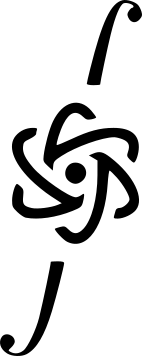
\includegraphics[height=2cm]{img-congreso/logo-congreso.png}
%\hspace*{7cm}~
%}

\logo{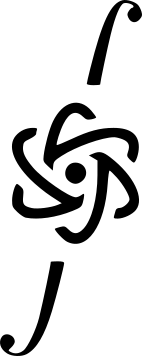
\includegraphics[height=3.5cm]{img-congreso/logo-congreso.png}
\hspace*{0.6cm}}
\institute[ECFM-USAC]{
	\inst{1}
	Escuela de Ciencias Físicas y Matemáticas\\
	Universidad de San Carlos de Guatemala
	\and
	\inst{2}
	Instituto de Física\\
	Universidad Nacional Autónoma de México} 
\date[VI Congreso Estudiantil]{28 de septiembre de 2020} 
 

\begin{document}

\section*{Título}
\begin{frame}[plain]
	\titlepage
	\begin{tikzpicture}[x=1mm,y=1mm,overlay,remember picture]
    \pgftransformshift{\pgfpointanchor{current page}{center}}
%    \node[inner sep=0pt] (usac) at (-50,30) %
%    {
\includegraphics[height=15mm]{images/ifunam}};
%    \node[inner sep=0pt] (ecfm) at (50,30) %
%    {
\includegraphics[height=15mm]{images/ecfmByN}};
    \node[inner sep=0pt] (congreso) at (45,-30) %
    {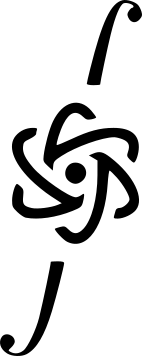
\includegraphics[height=20mm]{img-congreso/logo-congreso}};
  \end{tikzpicture}
\end{frame}

\logo{}

\begin{frame}
	\begin{figure}
		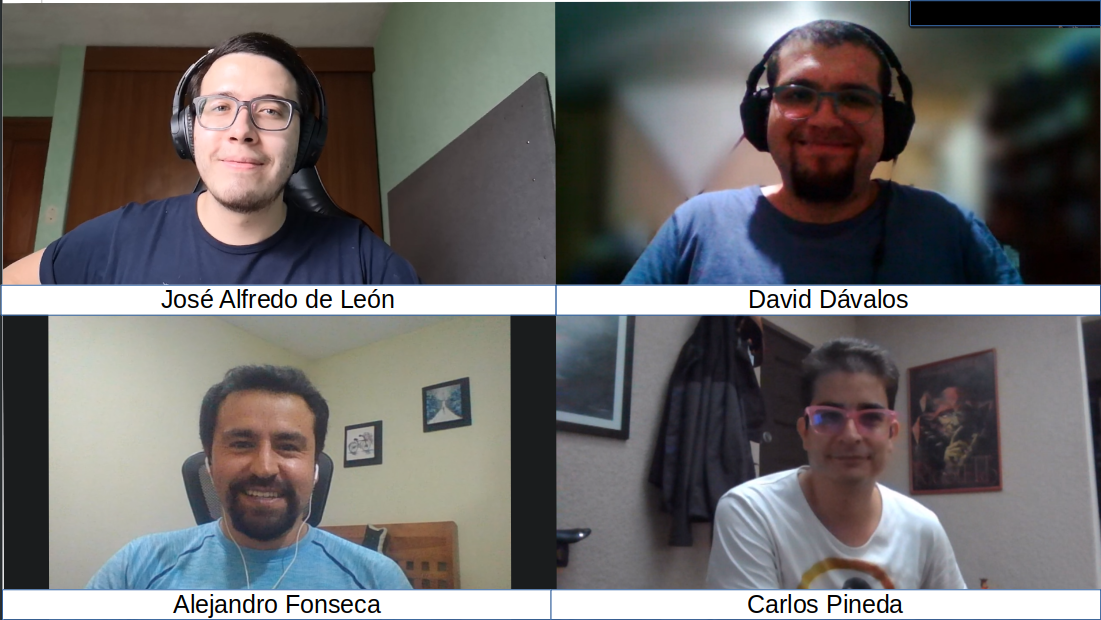
\includegraphics[width=\textwidth]{img-congreso/foto-grupo-1}
	\end{figure}
	\begin{tikzpicture}[x=1mm,y=1mm,overlay,remember picture]
    \pgftransformshift{\pgfpointanchor{current page}{center}}
    \node[inner sep=0pt] (usac) at (-45,-32) %
    {
\includegraphics[height=15mm]{images/ifunam}};
    \node[inner sep=0pt] (ecfm) at (47,-32) %
    {
\includegraphics[height=15mm]{images/ecfmByN}};
  \end{tikzpicture}
\end{frame}

\addtobeamertemplate{frametitle}{}{%
\begin{textblock*}{100mm}(.90\textwidth,6.9cm)
%\includegraphics[height=1.2cm]{logoECFM.png}
\end{textblock*}}

\section*{Esquema}
\begin{frame}{Esquema}
	\tableofcontents[hideallsubsections]
\end{frame}

\AtBeginSection[]
{
	\begin{frame}{Esquema}
		\tableofcontents[currentsection,hideallsubsections]
	\end{frame}
}

\section{Introducción}
\begin{frame}{Introducción}
		\only<2>{
		Estado de un sistema físico:
		\begin{figure}
			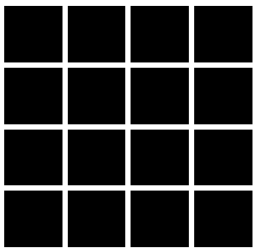
\includegraphics[height=3cm]{img-congreso/motivacion0}
		\end{figure}
		}
		\only<3-5>{
		\begin{tikzpicture}[x=1mm,y=1mm,overlay,remember picture]
			\pgftransformshift{\pgfpointanchor{current page}{center}}
			\node[inner sep=0pt] (usac) at (-30,10) %
			{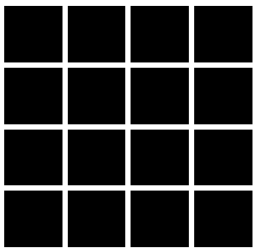
\includegraphics[height=3cm]{img-congreso/motivacion0}};
			\node[inner sep=0pt] (usac) at (30,10) %
			{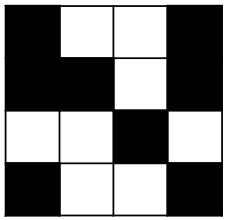
\includegraphics[height=3cm]{img-congreso/motivacion01}};
			\node[inner sep=0pt] (usac) at (-30,30) %
			{\text{estado inicial:}};
			\node[inner sep=0pt] (usac) at (30,30) %
			{\text{estado final:}};
		\end{tikzpicture}
		\vspace{5cm}
		}
		\only<4-5>{
		\begin{tikzpicture}[x=1mm,y=1mm,overlay,remember picture]
			\pgftransformshift{\pgfpointanchor{current page}{center}}
			\draw[thick, ->] (-15,10) -- (14,10);
			\node[inner sep=0pt] (usac) at (0,13) %
			{\text{¿evolución física?}};
		\end{tikzpicture}
		}
		\only<5>{
		\begin{itemize}
			\item Arena: mecańica cuántica
			\item Tipo de sistemas: abiertos (no ideales)
		\end{itemize}
		}
		\only<6>{
		Algunos posibles estados con la mitad de la información borrada:
		\begin{figure}
			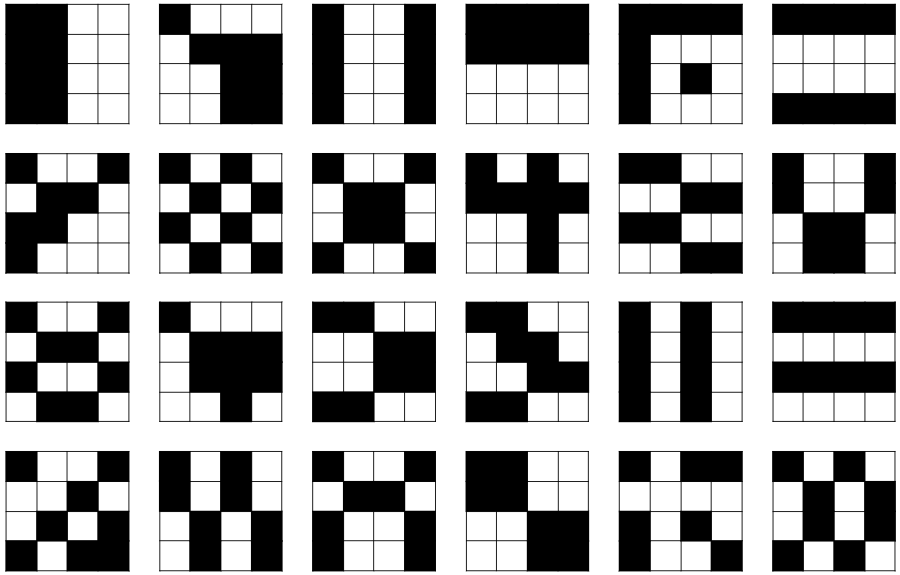
\includegraphics[height=6cm]{img-congreso/motivacion1}
		\end{figure}
		}
		\only<7>{
		Resultados de una evolución física {\colorbox{Red}{\color{Red}o}} y que no
		\colorbox{Black}{\color{Black}o}:
		\begin{figure}
			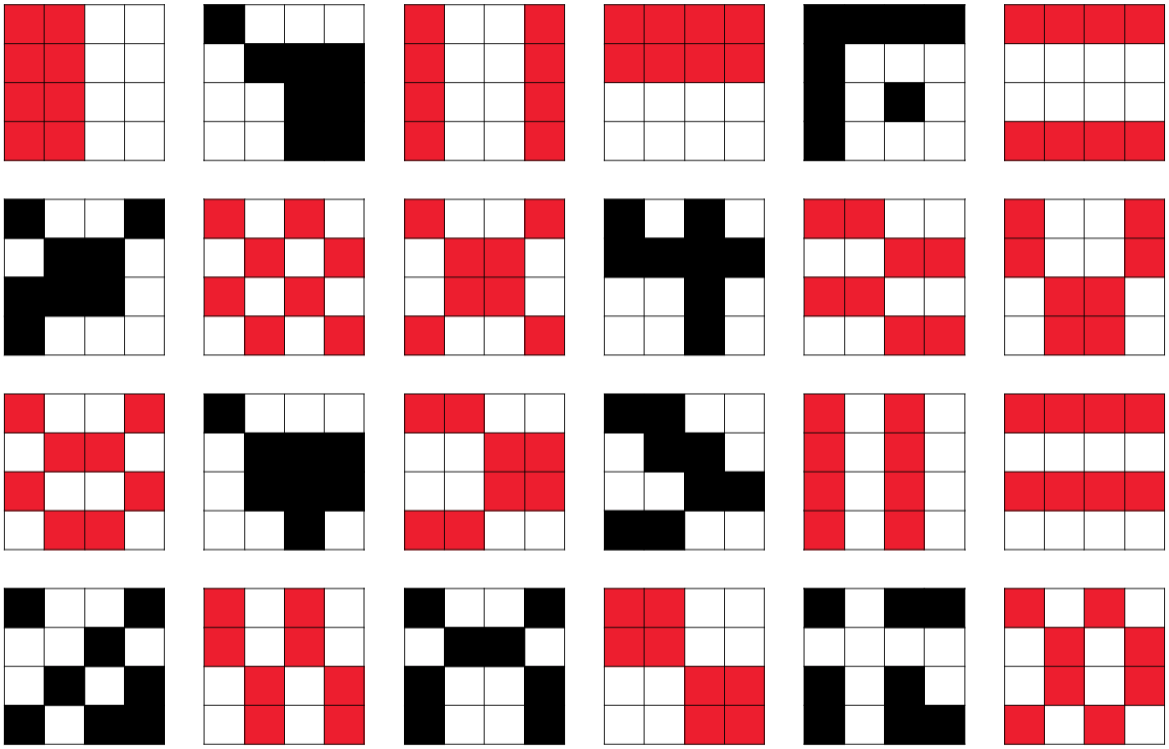
\includegraphics[height=6cm]{img-congreso/motivacion2}
		\end{figure} 
		}
		\only<8>{
		Resultados de una evolución física {\colorbox{Red}{\color{Red}o}} y que no
		\colorbox{Black}{\color{Black}o}:
		\begin{figure}
			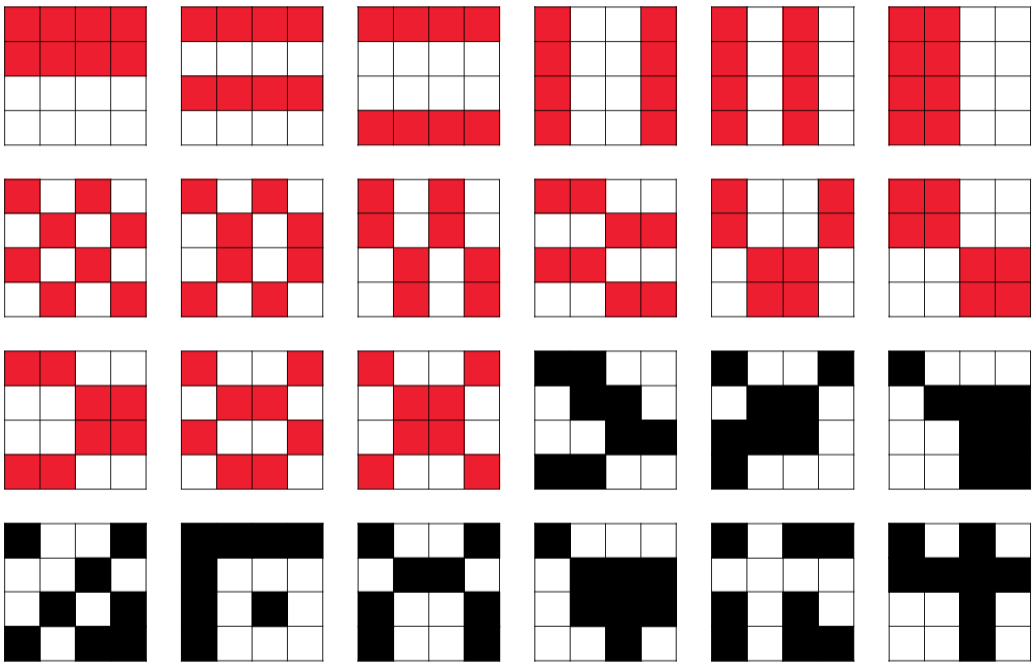
\includegraphics[height=6cm]{img-congreso/motivacion4}
		\end{figure} 
		}
		\only<9>{
		\begin{itemize}[label=$\textcolor{Blue}{\blacktriangleright}$]
			\item Operaciones que borran información de un estado
			\item Caracterizar cuáles de esas operaciones representan procesos
						físicos
		\end{itemize}
		}
\end{frame}




%\section{Introducción}
%
%\subsection{Información cuántica}
%\begin{frame}{¿Qué se estudia en Información cuántica?}\pause
%  ¿Es posible manipular y controlar sistemas cuánticos complejos?\newline	
%	De ser así, ¿qué implicaciones científicas	y tecnológicas tiene eso?\vfill
%	\pause
%	
%	Factorización en primos:
%	\begin{align*}
%		10 &=5 \times 2\\
%		24 &= 2 \times 2 \times 2 \times 3\\
%		231654687498461 &= \hspace*{1mm} ? \hspace*{1mm} \times 
%		\hspace*{1mm} ? \times \cdots	\times \hspace*{1mm} ?,
%	\end{align*}
%	\pause
%
%	En 1994, Peter Shor mostró que problemas difíciles en el mundo clásico son
%	problemas fáciles en el mundo cuántico.
%\end{frame}
%
%
%
%\begin{frame}{¿Qué se estudia en Información cuántica?}
%	\begin{columns}
%	\begin{column}{0.5\textwidth}
%		\onslide<1->{
%  	\begin{center}
%  		\textbf{Computadora clásica}
%  	\end{center}
%  	}
%  	\begin{itemize}[label=$\textcolor{Blue}{\blacktriangleright}$]
%  		\item<2-> Factorizar un número de 193 dígitos tomó 30 años de CPU (2.2 GHz). 
%  		\item<3-> Factorizar un número de 500 dígitos tomaría $10^{12}$ años de CPU.
%  	\end{itemize}
%	\end{column}
%	\begin{column}{0.5\textwidth} 
%		\onslide<1->{
%  	\begin{center}
%  		\textbf{Computadora cuántica}
%  	\end{center}
%  	}
%  	\begin{itemize}[label=$\textcolor{Blue}{\blacktriangleright}$]
%  		\item<2-> Se podría factorizar un número de 193 dígitos en 0.1 s.
%  		\item<3-> Se podría factorizar un número de 500 dígitos en 2s. 
%  	\end{itemize}
%  	\vspace{0.1cm}
%	\end{column}
%	\end{columns}
%	\vfill
%	\onslide<4->{
%	Para caracterizar esta ventaja teórica abrumadora entre la computación cuántica
%	y clásica John Preskill acuñó el término \textbf{supremacía cuántica}.}
%\end{frame}

%\section{Idea fundamental}
%\begin{frame}{Idea fundamental}
%	\centering
%	\LARGE  
%  \begin{columns}
%  	\begin{column}{0.38\textwidth}
%  		\centering
%  		estados físicos de qubits
%  	\end{column}
%  	\begin{column}{0.22\textwidth}
%  		\newline
%  		$\underset{\text{proceso físico}}{\mbox{\Huge $
%  		\mathbf{\longmapsto}$}}$
%  	\end{column}
%  	\begin{column}{0.42\textwidth}
%  		\centering
%  		otros estados físicos de qubits
%  	\end{column}
%  \end{columns}\vfill \pause
%  
%  \normalsize
%    \begin{columns}
%  	\begin{column}{0.25\textwidth}
%  	\end{column}
%  	\begin{column}{0.5\textwidth}
%		  \begin{itemize}[label=$\textcolor{Blue}{\blacktriangleright}$]
%		  	\item ¿qubits?
%		  	\item ¿estados?
%		  	\item ¿cuál proceso físico?
%		  	\item ¿qué otros estados?
%		  \end{itemize}
%  	\end{column}
%  	\begin{column}{0.1\textwidth}
%  	\end{column}
%  \end{columns}
%\end{frame}



\section{Marco teórico}

\subsection{Qubit}
\begin{frame}{Qubits}\pause	
	\begin{columns}
  	\begin{column}{0.48\textwidth}
  		\begin{itemize}[label=$\textcolor{Blue}{\blacktriangleright}$]
				\item<2-> Análogos cuánticos de los bits.
							
				\item<4-> \alert{$\ket{\Psi} = \alpha \ket{0} + \beta \ket{1}$},
							vector en $\mathcal{H}=\mathbb{C}^2$ 
							
				\item<5-> $n$ qubits: espacio vectorial complejo de dimensión $2^n$, 
									$\underbrace{\mathbb{C}^2\otimes\ldots\otimes\mathbb{C}^2}
									_{n\ \text{veces}}$
	\end{itemize}
  	\end{column}
  	\begin{column}{0.48\textwidth}
  		\centering
			\only<2>{\textbf{Bit clásico}}
			\only<2>{
 			\begin{figure}
				\centering
				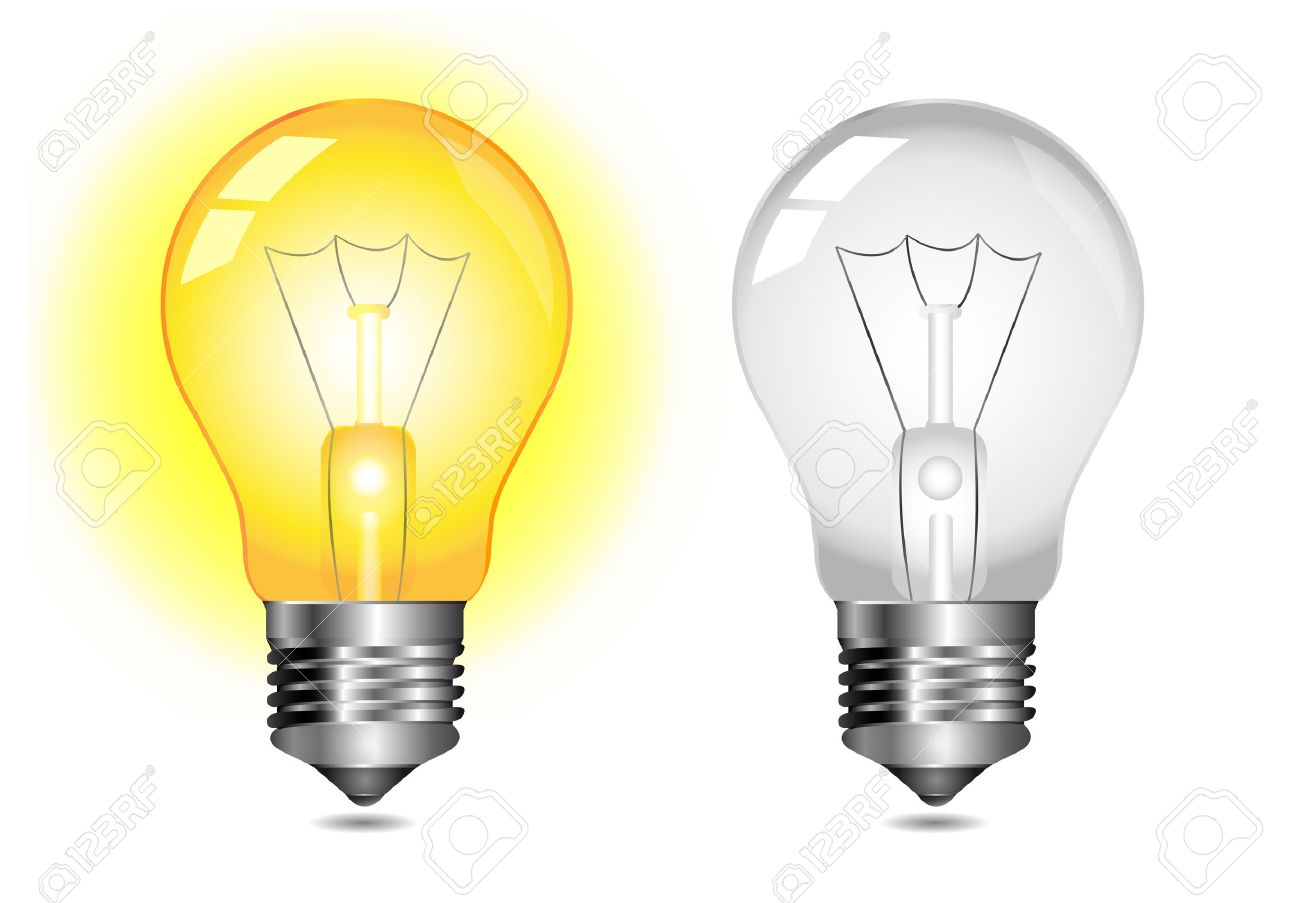
\includegraphics[height=3cm]{img-congreso/bulbs}
			\end{figure} 
			\hspace{0.2cm} encendido: 1 \hspace{0.2cm} apagado: 0 \hfill}
			\only<3->{\textbf{Qubit}} 
			\only<3->{
		  \begin{figure}
				\centering
				\hspace{.5cm}
				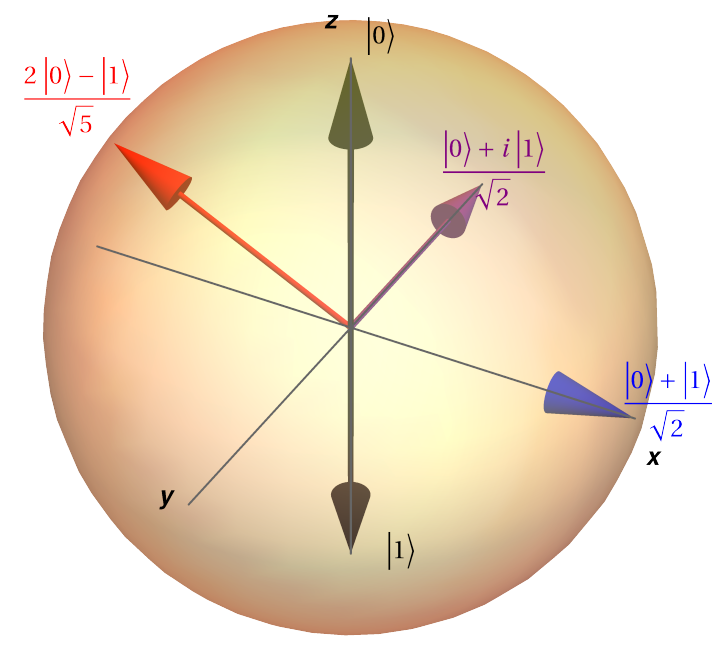
\includegraphics[height=4cm]{img-congreso/bloch}\newline
				\alert{Bola de Bloch}
			\end{figure}				
			}
  	\end{column}
  \end{columns}	

\end{frame}



%\begin{frame}
%	2 características hacen a los qubits hacen fundamentalmente 
%	distintos	de los bits: 
%	\newline
%	\begin{itemize}[label=$\textcolor{Blue}{\blacktriangleright}$]
%		\item \textbf{Superposición}: 1 qubit puede estar `encendido' y 
%					`apagado' al mismo tiempo,
%					\begin{align*}
%						\ket{\Psi} = \alpha \ket{0} + \beta \ket{1};
%					\end{align*}
%					en cada estado con probabilidad \alert{$\abs{\alpha}^2$} y 
%					\alert{$\abs{\beta}^2$},
%					respectivamente.
%		
%		\item \textbf{Entrelazamiento}: \textit{`El todo es más que la suma
%					de sus partes',}
%					\begin{align*}
%						\mathcal{H}_P\otimes \mathcal{H}_E.
%					\end{align*}
%	\end{itemize}
%\end{frame}



%\begin{frame}
%	Un qubit es cualquier sistema cuántico de dos niveles.
%	\begin{columns}
%  	\begin{column}{0.48\textwidth}
%  			\begin{figure}
%					\centering
%					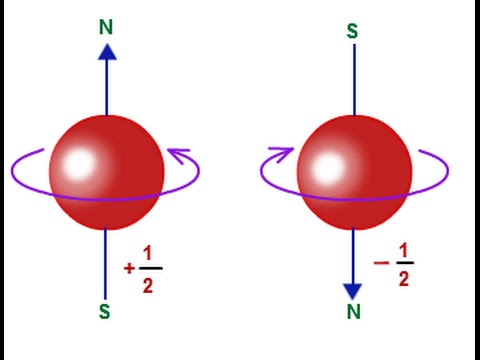
\includegraphics[height=0.4\textheight]{img-congreso/e-spin}
%					\caption{Partículas de espín $\frac{1}{2}$.}
%				\end{figure}
%  	\end{column}
%  	\begin{column}{0.48\textwidth}
%		  \begin{figure}
%					\centering
%					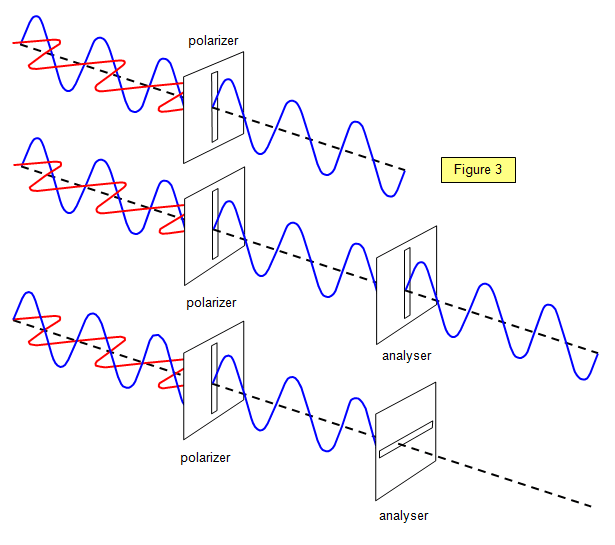
\includegraphics[height=0.4\textheight]{img-congreso/photon}
%					\caption{Polarización de fotones.}
%				\end{figure}
%  	\end{column}
%  \end{columns}
%\end{frame}



\subsection{Matriz de densidad}
\begin{frame}{Matriz de densidad}
	\only<2->{
	Toda la información del estado de un sistema cuántico está 
	codificada en su \alert{matriz	de densidad $\rho$},
	\[
		\rho = \dyad{\Psi}{\Psi}.
	\]
	}
	\only<2>{
	\vspace{5cm}
	}

	\begin{columns}
		\only<3->{
		\begin{column}{0.5\textwidth}
			Para 1 qubit:
			\begin{align*}
				\rho &= \frac{\mathbb{1} + \vec{r}\vdot \vec{\sigma}}{2}\\
				\rho &= \frac{\alert{(1)}\mathbb{1} + \alert{r_x}\sigma _x 
				+ \alert{r_y}\sigma_y + \alert{r_z}\sigma_z}{2},
			\end{align*}
			donde $\vec{r}$ es el vector de Bloch ($\norm{\vec{r}
			\hspace{2pt}}
			\leq 1$) y $\sigma _i$ son las matrices de Pauli.
		\end{column}
		}
		\begin{column}{0.45\textwidth}
			\only<3>{
			\begin{figure}
				\centering
				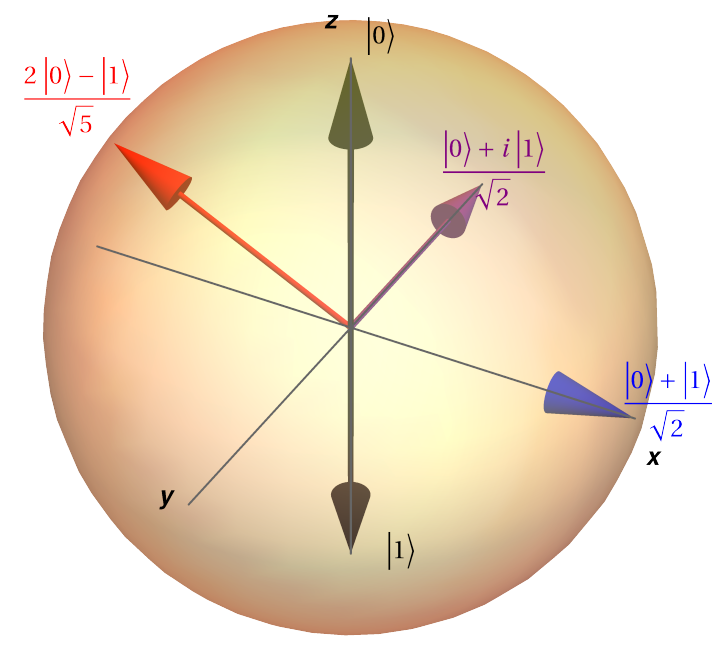
\includegraphics[height=4cm]{img-congreso/bloch}
			\end{figure}
			}
		\only<4>{
		\noindent Para n qubits:
		\begin{align*}
			\rho = \frac{1}{2^n}\mathbb{1} + \sum _{i=1}^{2^{2n}-1}\tau _i\Omega _i,
		\end{align*}
		de donde vamos a ocupar a los productos tensoriales de las matrices de Pauli
		como los operadores $\Omega _i$.
		}
		\end{column}
\end{columns}
\end{frame}



\subsection{Canales cuánticos}
\begin{frame}{Sistemas cuánticos abiertos}
	Los sistemas cuánticos que pueden estar en interacción con su 
	entorno se conocen como \textbf{sistemas cuánticos abiertos};\pause
	\begin{align*}
		\mathcal{H}_{\text{total}}=\mathcal{H}_P\otimes \mathcal{H}_E.
	\end{align*}\pause
	
	El formalismo de los \textbf{canales cuánticos} es una herramienta matemática
	que se utiliza para describir la evolución de los sistemas cuánticos abiertos. 
	\begin{figure}
	\centering
		\begin{tikzpicture}
			\draw[thick, ->] (-1,1.5) node[anchor=east] {\huge $\rho$} -- (-0.05,1.5);
			\draw[thick] (0,0) rectangle (2,3);
			\node[anchor=north,inner sep=0] at (1,1.8) {\Huge $\Phi$};
			\draw[thick, ->] (2.05,1.5) -- (3,1.5) node[anchor=west] {\huge $\rho'$};
		\end{tikzpicture}
		%\caption{Ilustración de la evolución de un estado cuántico a través de
		%un canal cuántico.}
	\end{figure}
\end{frame}


\begin{frame}{Canales cuánticos}
	Un canal cuántico es un mapeo lineal que transforma a la matriz de 
	densidad del sistema como
	\begin{align*}
		\rho ' = \Phi \qty(\rho),
	\end{align*}
	donde $\Phi$ representa matemáticamente la evolución física entre 
	un estado inicial y un estado final del sistema.\vfill \pause
	
	Para que $\Phi$ sea un canal cuántico no es suficiente con que sea una
	transformación de matrices de densidad en	matrices de densidad. 
	Adicionalmente, se requiere la condición de	\textbf{completa positividad}.
\end{frame}



\subsection{Canales cuánticos de 1 qubit}

\begin{frame}
	\centering
	{\LARGE
	Algunos canales cuánticos de 1 qubit...}\vfill
	
	\begin{itemize}[label=$\textcolor{Blue}{\blacktriangleright}$]
		\item Se parametrizan en función de una probabilidad $p$ con la que 
					podría ocurrir la acción del canal.
		\item Acción de un canal cuántico: deformación de la bola de Bloch.
	\end{itemize}
\end{frame}

%\begin{frame}{Inversión de bit}
%	\begin{columns}
%		\begin{column}{0.48\textwidth}
%			\begin{figure}
%				\centering
%				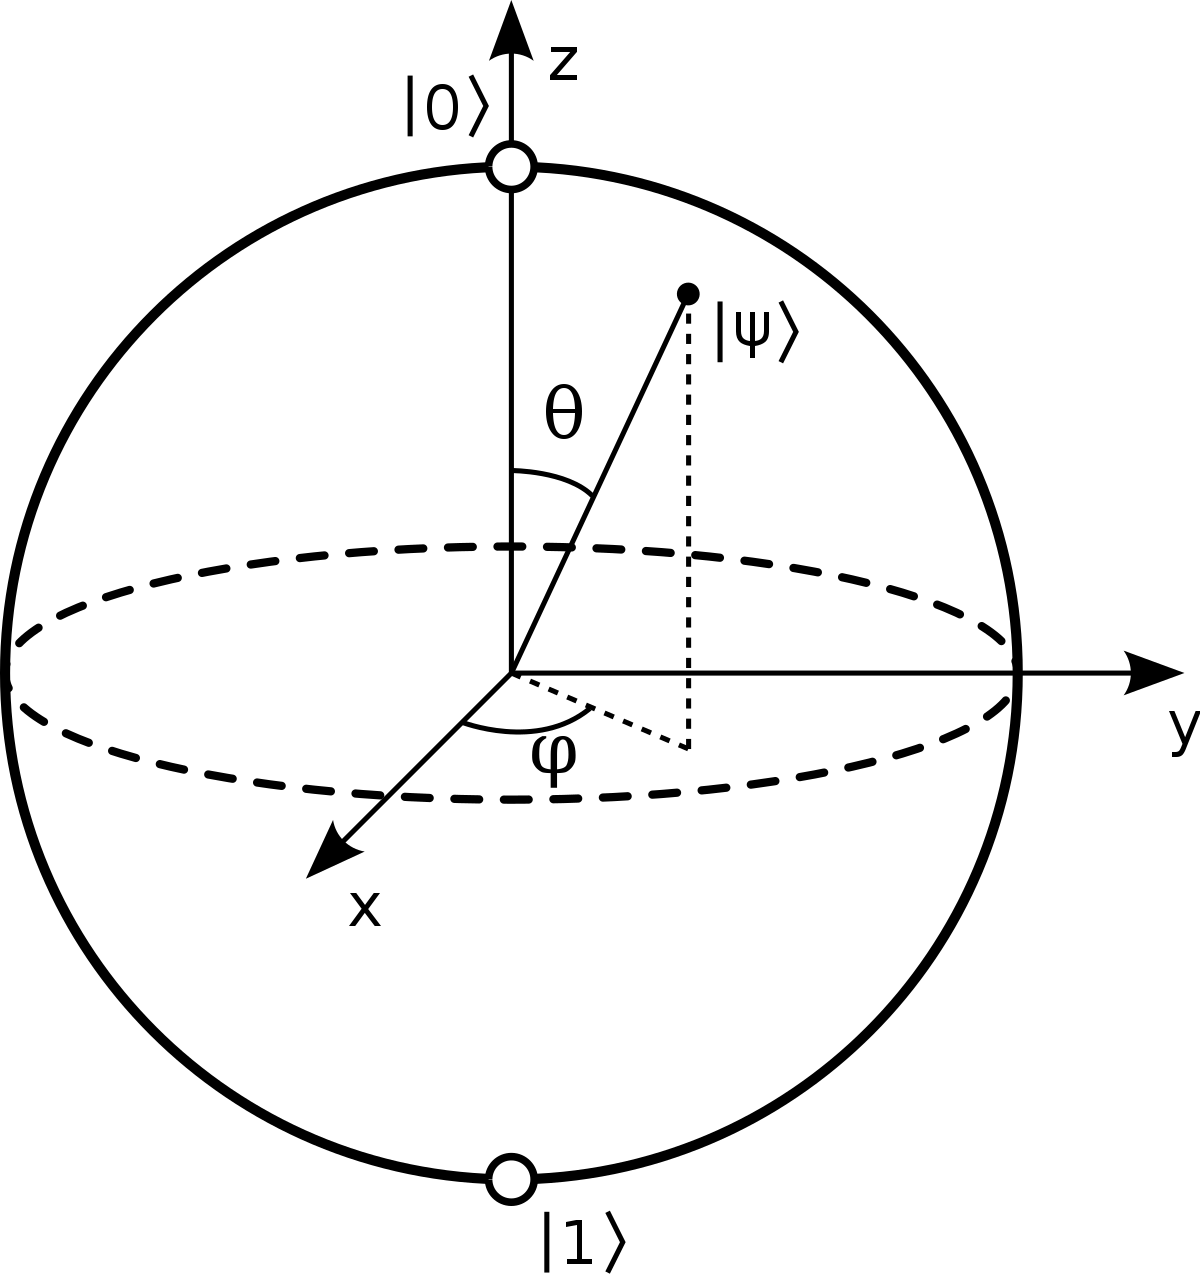
\includegraphics[height=0.5\textheight]{blochSphere.pdf}
%				%\caption{Todos los puntos en la esfera de Bloch (dentro y fuera)
%				%representan estados de 1 qubit.}
%			\end{figure}
%		\end{column}
%		\begin{column}{0.05\textwidth}
%			\vfill
%			\centering	
%			\huge
%			$\longrightarrow$
%			\vfill
%		\end{column}
%		\begin{column}{0.48\textwidth}
%				\begin{figure}
%					\centering
%					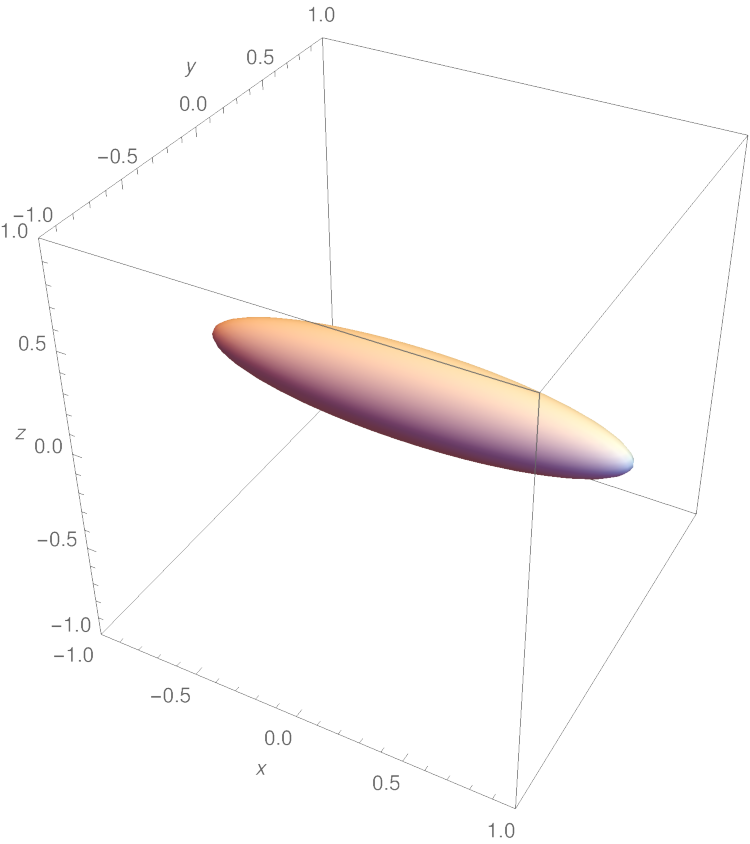
\includegraphics[height=0.5\textheight]{img-congreso/bit-flip.pdf}
%					%\caption{Bit flip, p=0.4}
%				\end{figure}\vfill
%		\end{column}
%	\end{columns}
%\end{frame}
%
%
%\begin{frame}{Inversión de fase}
%\begin{columns}
%		\begin{column}{0.48\linewidth}
%			\begin{figure}
%				\centering
%				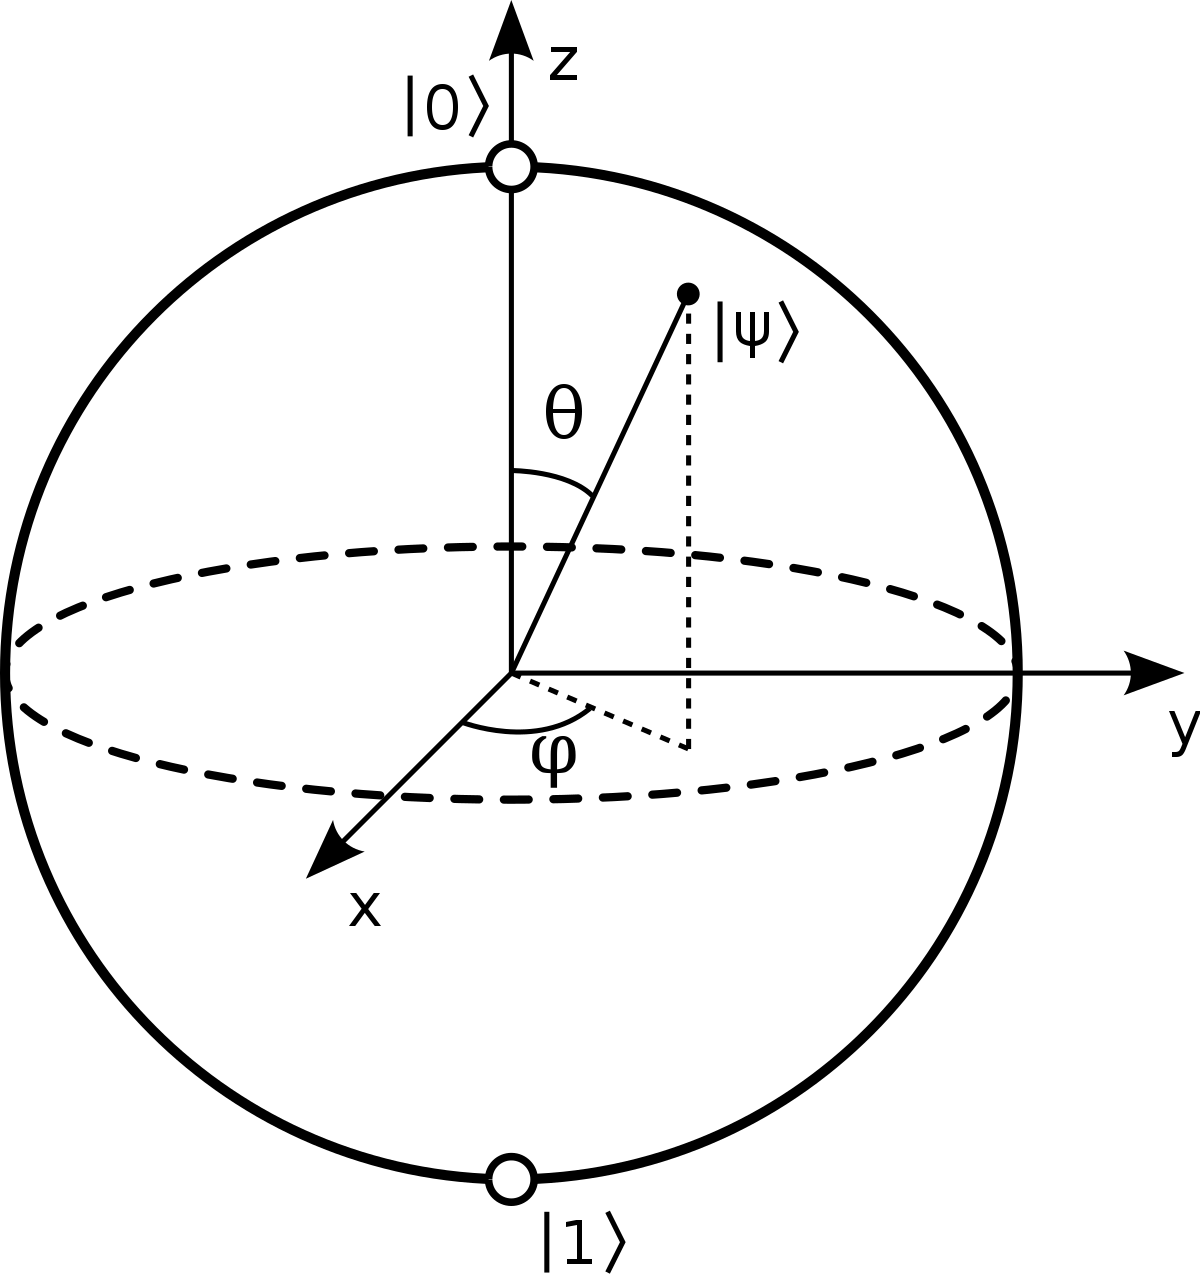
\includegraphics[height=0.5\textheight]{blochSphere.pdf}
%				%\caption{Todos los puntos en la esfera de Bloch (dentro y fuera)
%				%representan estados de 1 qubit.}
%			\end{figure}
%	\end{column}
%		\begin{column}{0.05\linewidth}
%			\centering	
%			\huge
%			$\longrightarrow$
%		\end{column}
%		\begin{column}{0.48\linewidth}
%			\begin{figure}
%				\centering
%				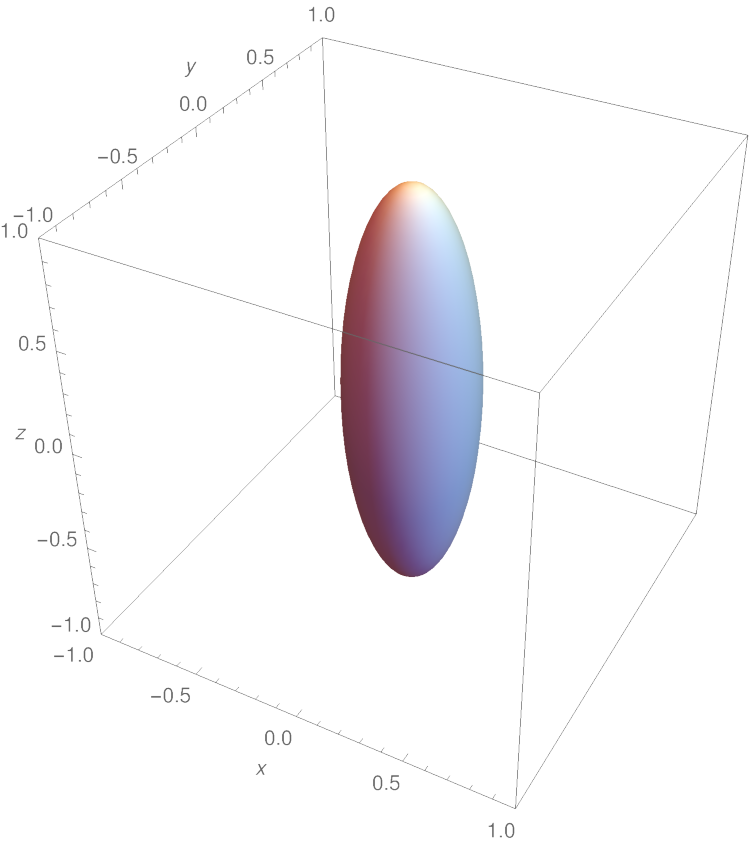
\includegraphics[height=0.5\textheight]{img-congreso/phase-flip.pdf}
%				%\caption{Phase flip, p=0.35}
%			\end{figure}
%	\end{column}
%\end{columns}
%\end{frame}
%
%
%
%\begin{frame}{Inversión de fase de bit}
%	\begin{columns}
%		\begin{column}{0.48\linewidth}
%			\begin{figure}
%				\centering
%				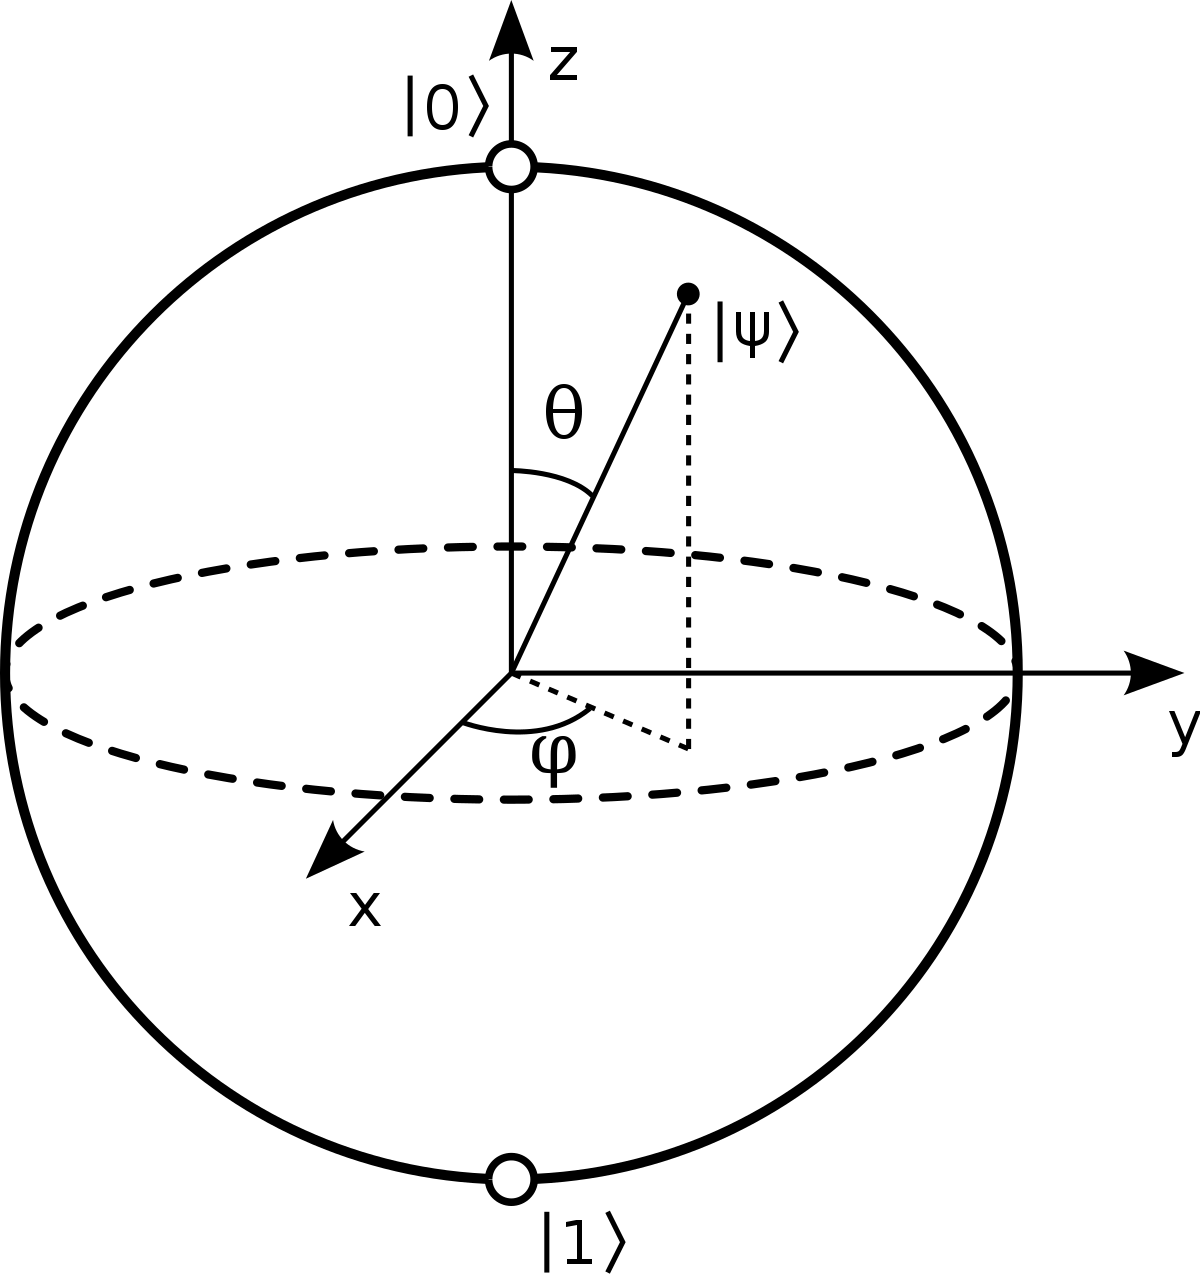
\includegraphics[height=0.5\textheight]{blochSphere.pdf}
%				%\caption{Todos los puntos en la esfera de Bloch (dentro y fuera)
%				%representan estados de 1 qubit.}
%			\end{figure}
%		\end{column}
%		\begin{column}{0.05\linewidth}
%			\centering	
%			\huge
%			$\longrightarrow$
%		\end{column}
%		\begin{column}{0.48\linewidth}
%				\begin{figure}
%					\centering
%					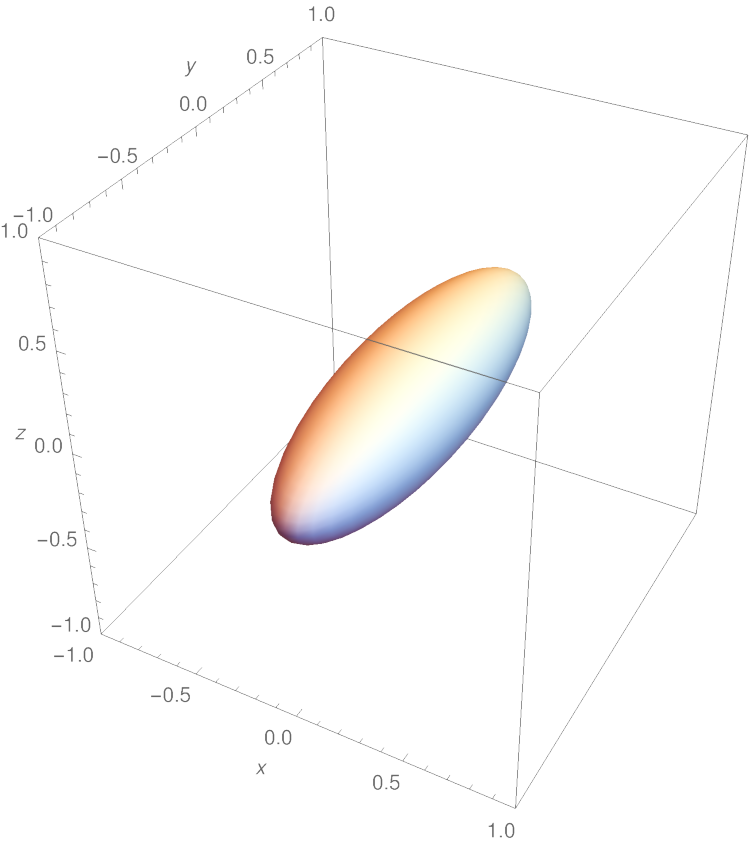
\includegraphics[height=0.5\textheight]{img-congreso/bit-phase-flip.pdf}
%					%\caption{Bit phase flip. p=0.35}
%				\end{figure}
%		\end{column}
%	\end{columns}
%\end{frame}
%
%
%
%\begin{frame}{Depolarizante}
%	\begin{columns}
%		\begin{column}{0.48\linewidth}
%			\begin{figure}
%				\centering
%				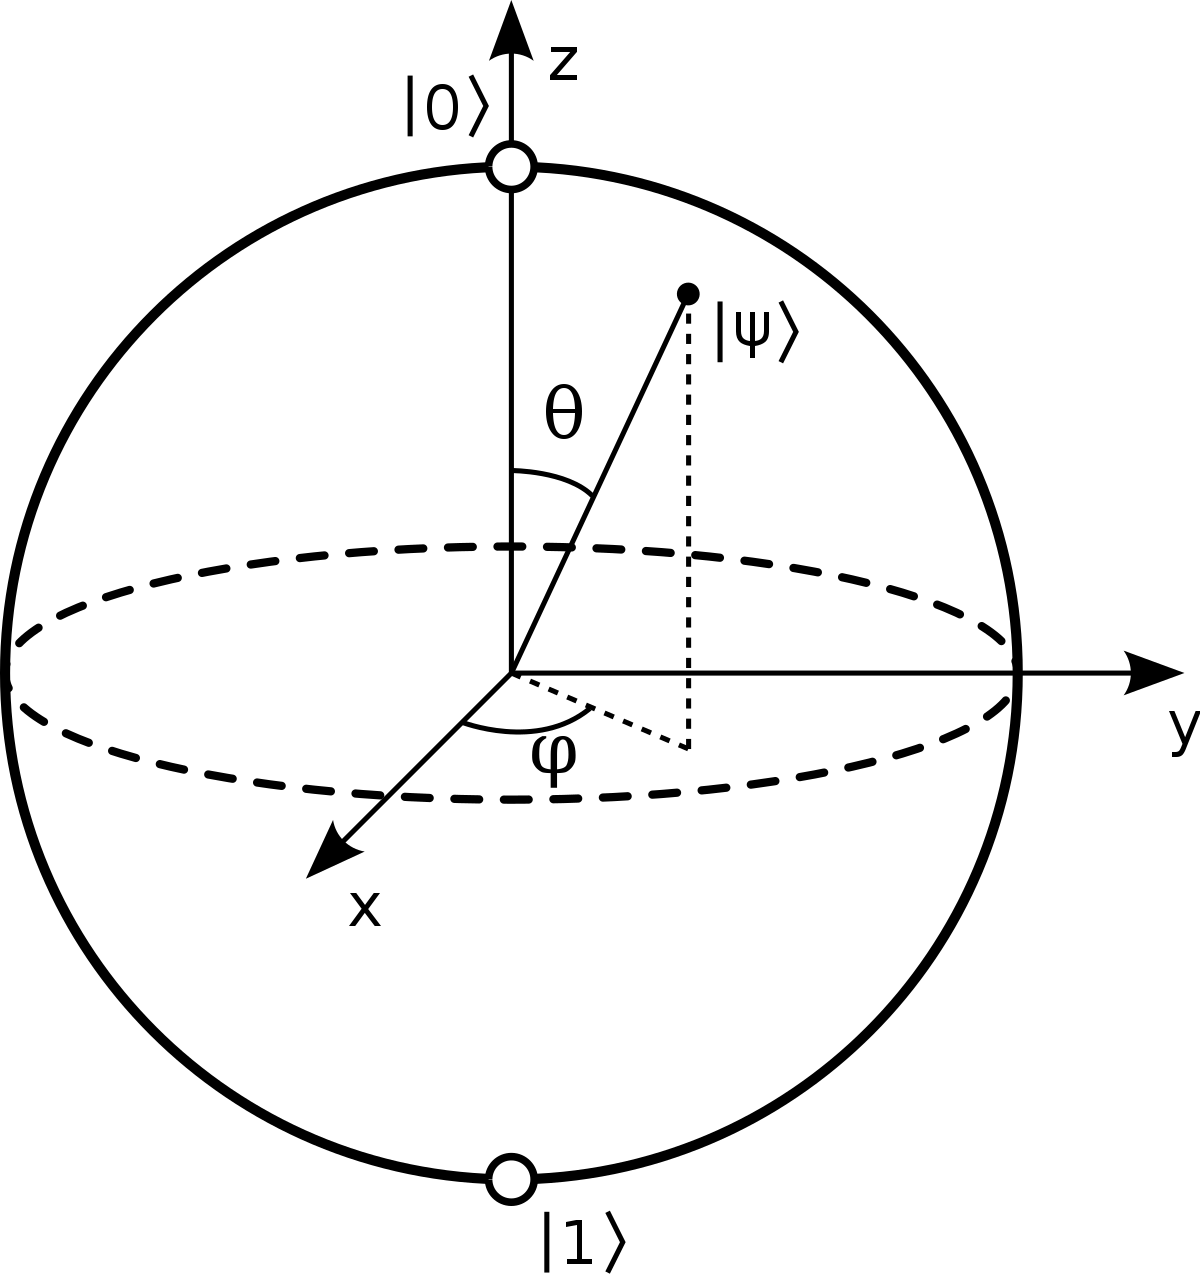
\includegraphics[height=0.5\textheight]{blochSphere.pdf}
%				%\caption{Todos los puntos en la esfera de Bloch (dentro y fuera)
%				%representan estados de 1 qubit.}
%			\end{figure}
%		\end{column}
%		\begin{column}{0.05\linewidth}
%			\centering	
%			\huge
%			$\longrightarrow$
%		\end{column}
%		\begin{column}{0.5\linewidth}
%			\begin{figure}
%				\centering
%				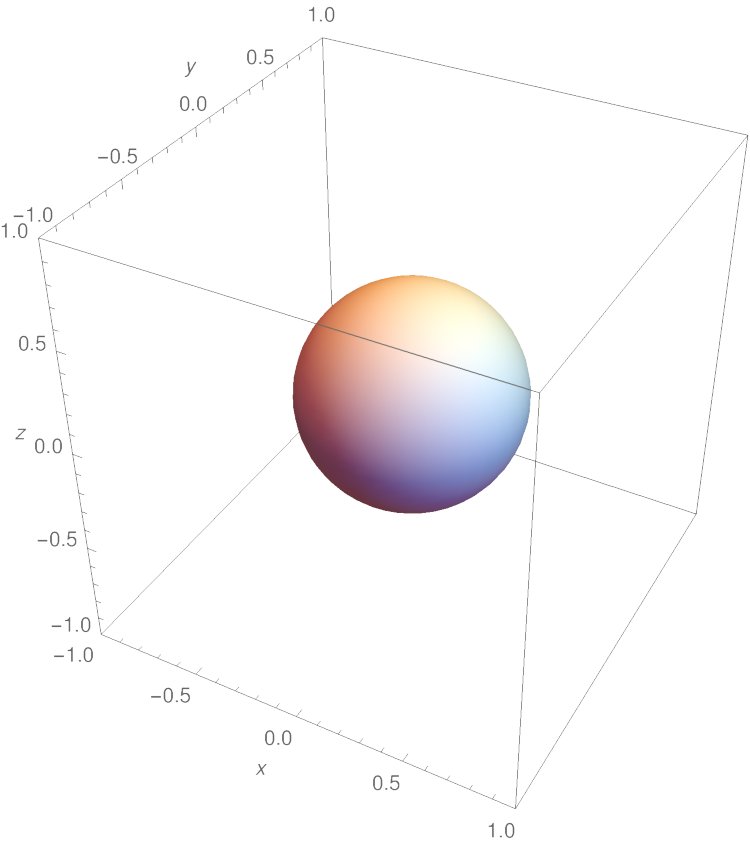
\includegraphics[height=0.48\textheight]{img-congreso/depolarizing.pdf}
%				%\caption{Depolarizante. p=0.35}
%			\end{figure}
%		\end{column}
%	\end{columns}
%\end{frame}

\subsection{}
\begin{frame}%{En resumen:}
	\textbf{En resumen:}
	\begin{itemize}[label=$\textcolor{Blue}{\blacktriangleright}$]
		\item Un \alert{qubit} es un sistema cuántico de dos niveles.
		\item La \alert{matriz de densidad $\rho$} es una herramienta para 
		describir	a un estado cuántico.
		\item Los \alert{sistemas cuánticos abiertos} son sistemas que interactúan  
		con su entorno.
		\item Los \alert{canales cuánticos} son una manera de de describir la 
		dinámica de los sistemas abiertos.
	\end{itemize}
\end{frame}



\section{Mapeos proyectivos}



\subsection*{}
\begin{frame}{Planteamiento del problema}
	Para un sistema de $n$ qubits ¿cómo se caracterizan los canales cuánticos del resto de los 
	mapeos que borran componentes	arbitrarias de la matriz de densidad?
\end{frame}



\subsection{1 qubit}
\begin{frame}{1 qubit}
	\only<1>{
	¿Cuáles de los mapeos que borran componentes de la matriz de densidad $\rho$
	de 1 qubit son canales cuánticos?
	
	\begin{columns}
		\begin{column}{0.5\textwidth}
			\begin{align*}
				\rho &= \frac{\alert{r_0}\mathbb{1} + \alert{r_x}\sigma _x 
				+ \alert{r_y}\sigma_y + \alert{r_z}\sigma_z}{2},
			\end{align*}
			con $r_0=1$.
		\end{column}
		\begin{column}{0.45\textwidth}
			\begin{figure}
				\centering
				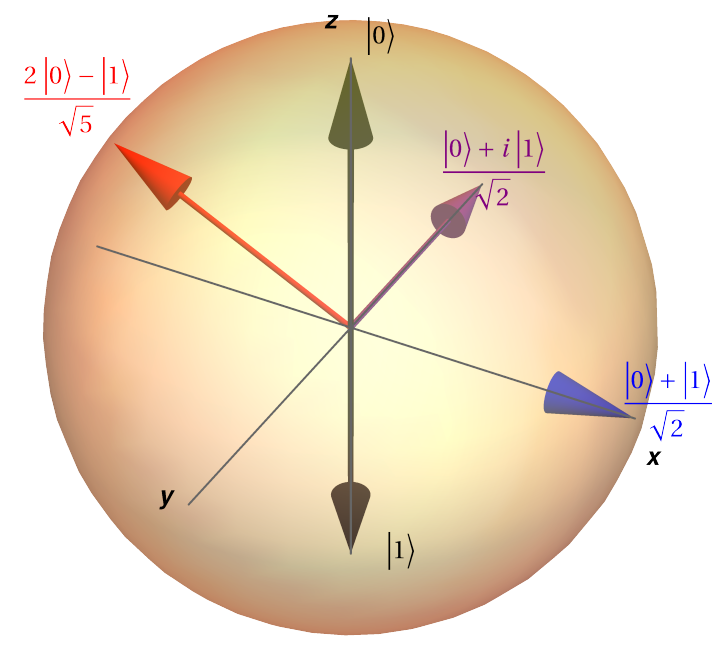
\includegraphics[height=4cm]{img-congreso/bloch}
			\end{figure}
		\end{column}
	\end{columns}
	}
	
	\only<2>{
	Dejar intacta la bola de Bloch:
	\begin{columns}
		\begin{column}{0.48\linewidth}
			\begin{figure}
				\centering
				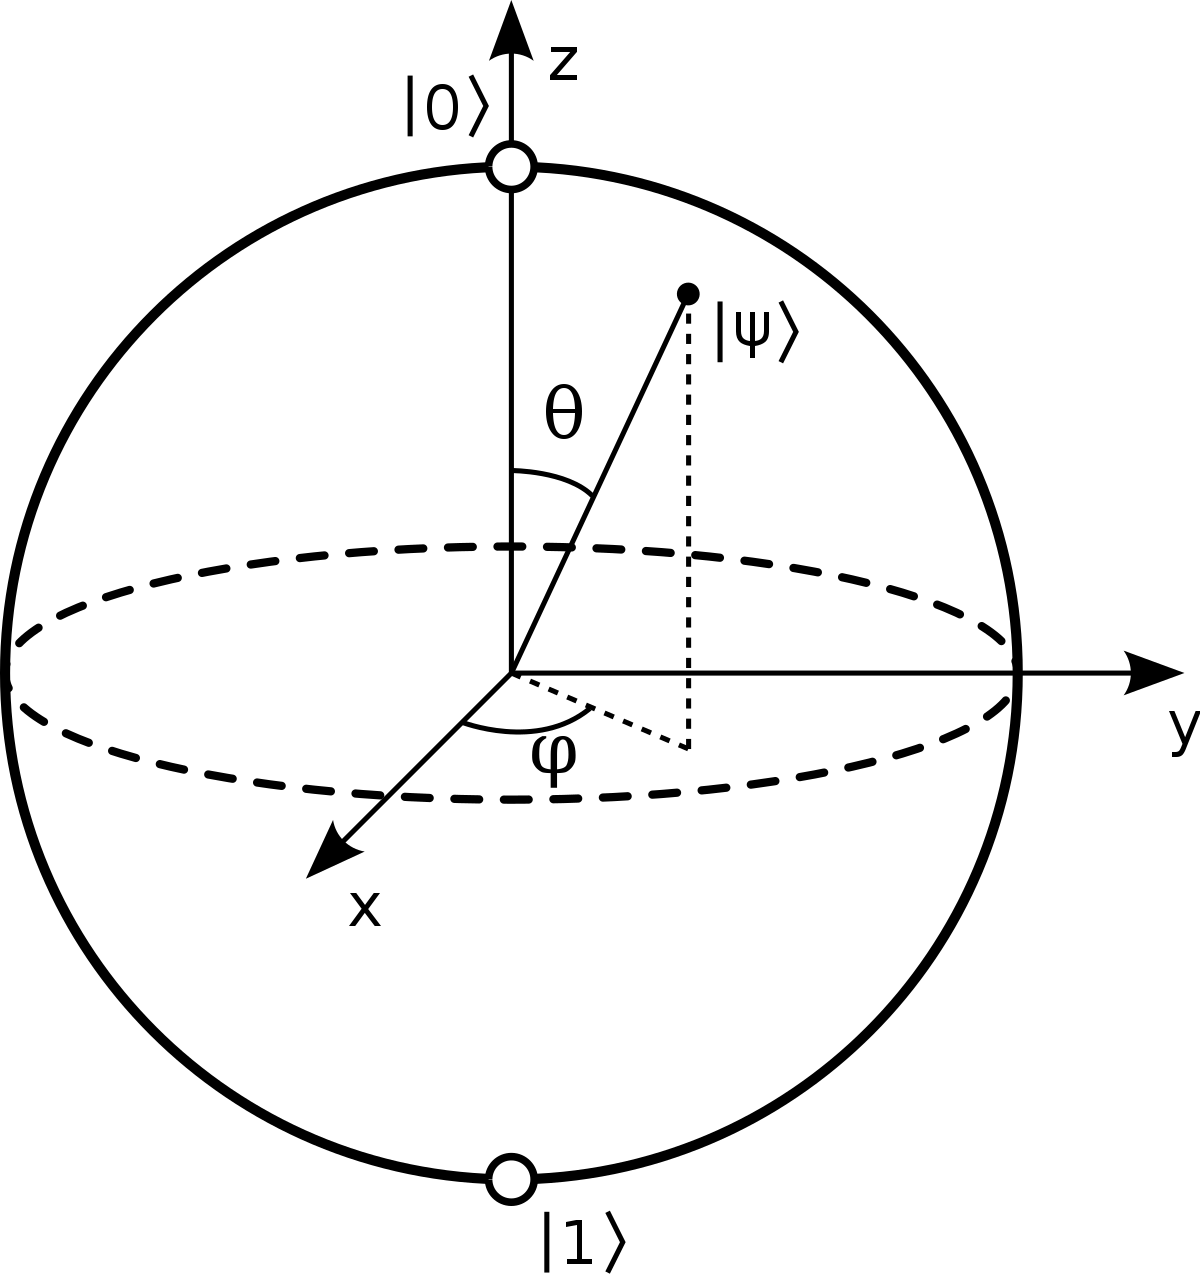
\includegraphics[height=0.5\textheight]{blochSphere.pdf}
			\end{figure}
		\end{column}
		\begin{column}{0.05\linewidth}
			\centering	
			\huge
			\colorbox{YellowGreen}{$\longrightarrow$}
		\end{column}
		\begin{column}{0.5\linewidth}
			\begin{figure}
				\centering
				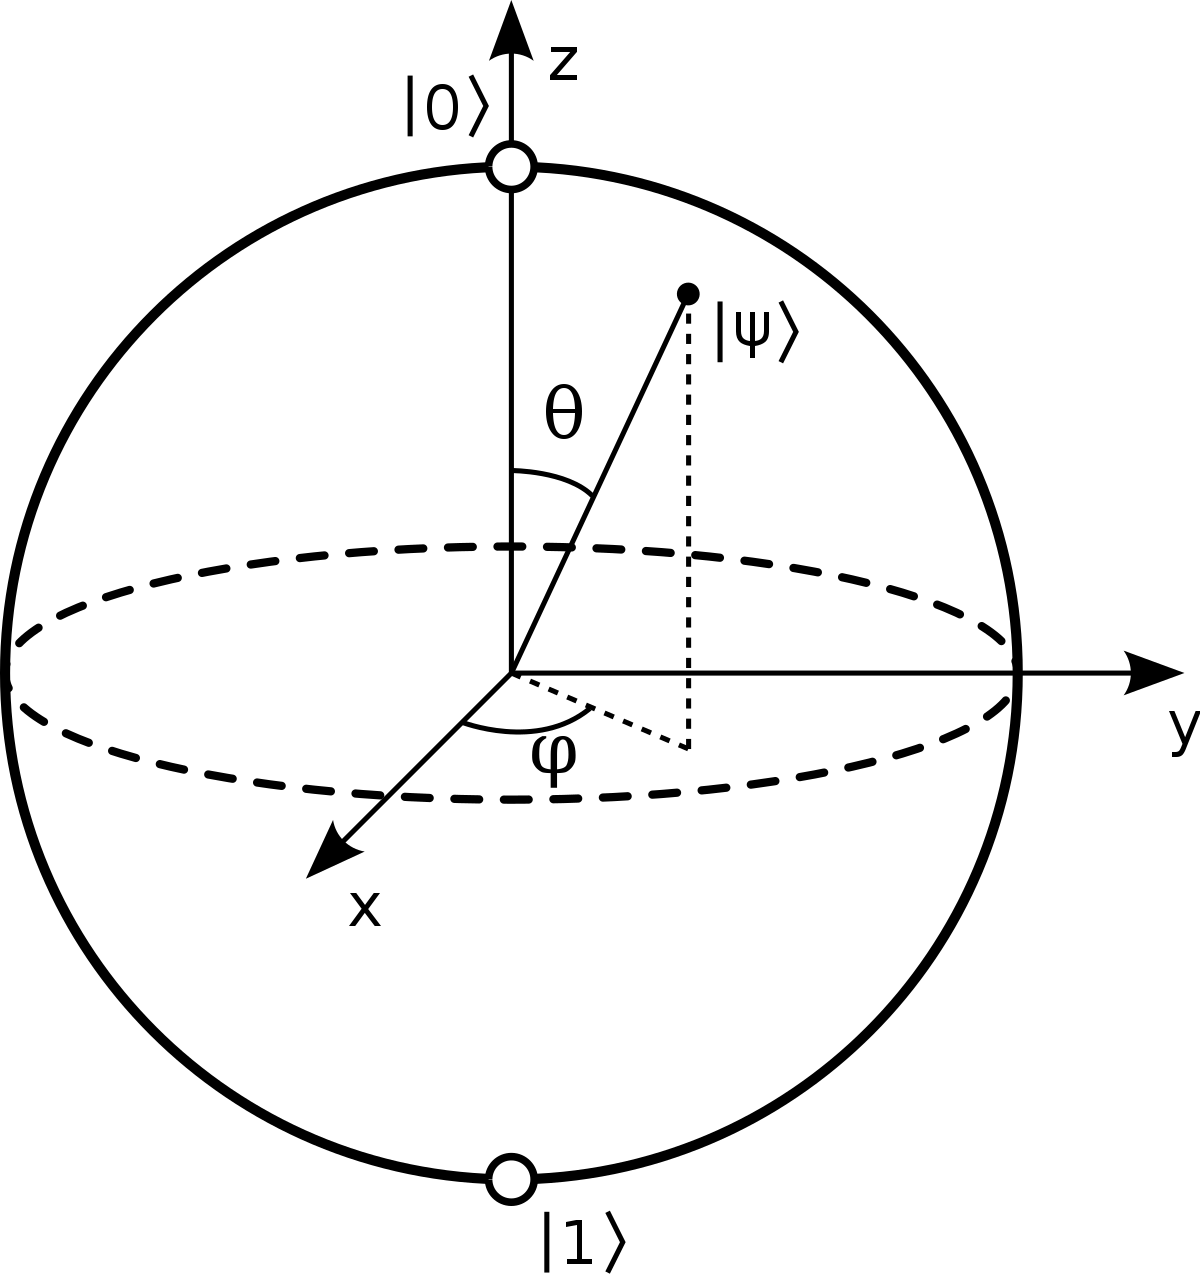
\includegraphics[height=0.48\textheight]{blochSphere.pdf}
			\end{figure}
		\end{column}
	\end{columns}
	\begin{align*}
		\colorbox{YellowGreen}{$\qty(r_x,r_y,r_z) 
		\longrightarrow \qty(r_x,r_y,r_z)$} 
	\end{align*}
	}
	
	\only<3>{
	Deformar la bola de Bloch en un disco:
	\begin{columns}
		\begin{column}{0.48\linewidth}
			\begin{figure}
				\centering
				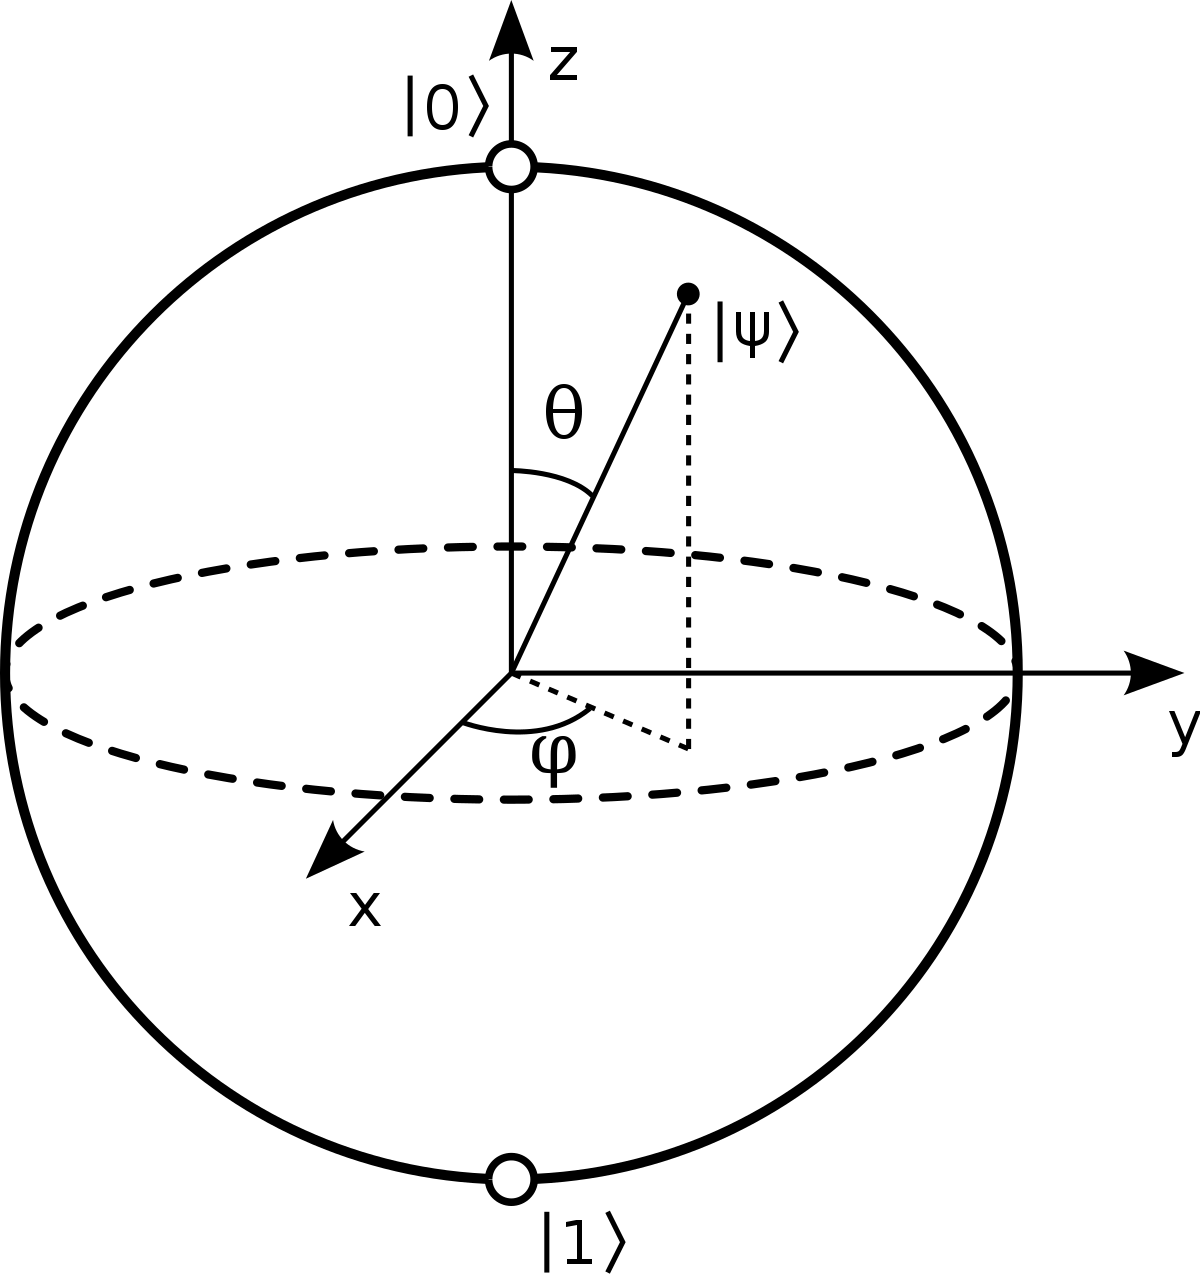
\includegraphics[height=0.5\textheight]{blochSphere.pdf}
			\end{figure}
		\end{column}
		\begin{column}{0.05\linewidth}
			\centering	
			\huge
			\colorbox{Red}{$\longrightarrow$}
		\end{column}
		\begin{column}{0.5\linewidth}
			\begin{figure}
				\centering
				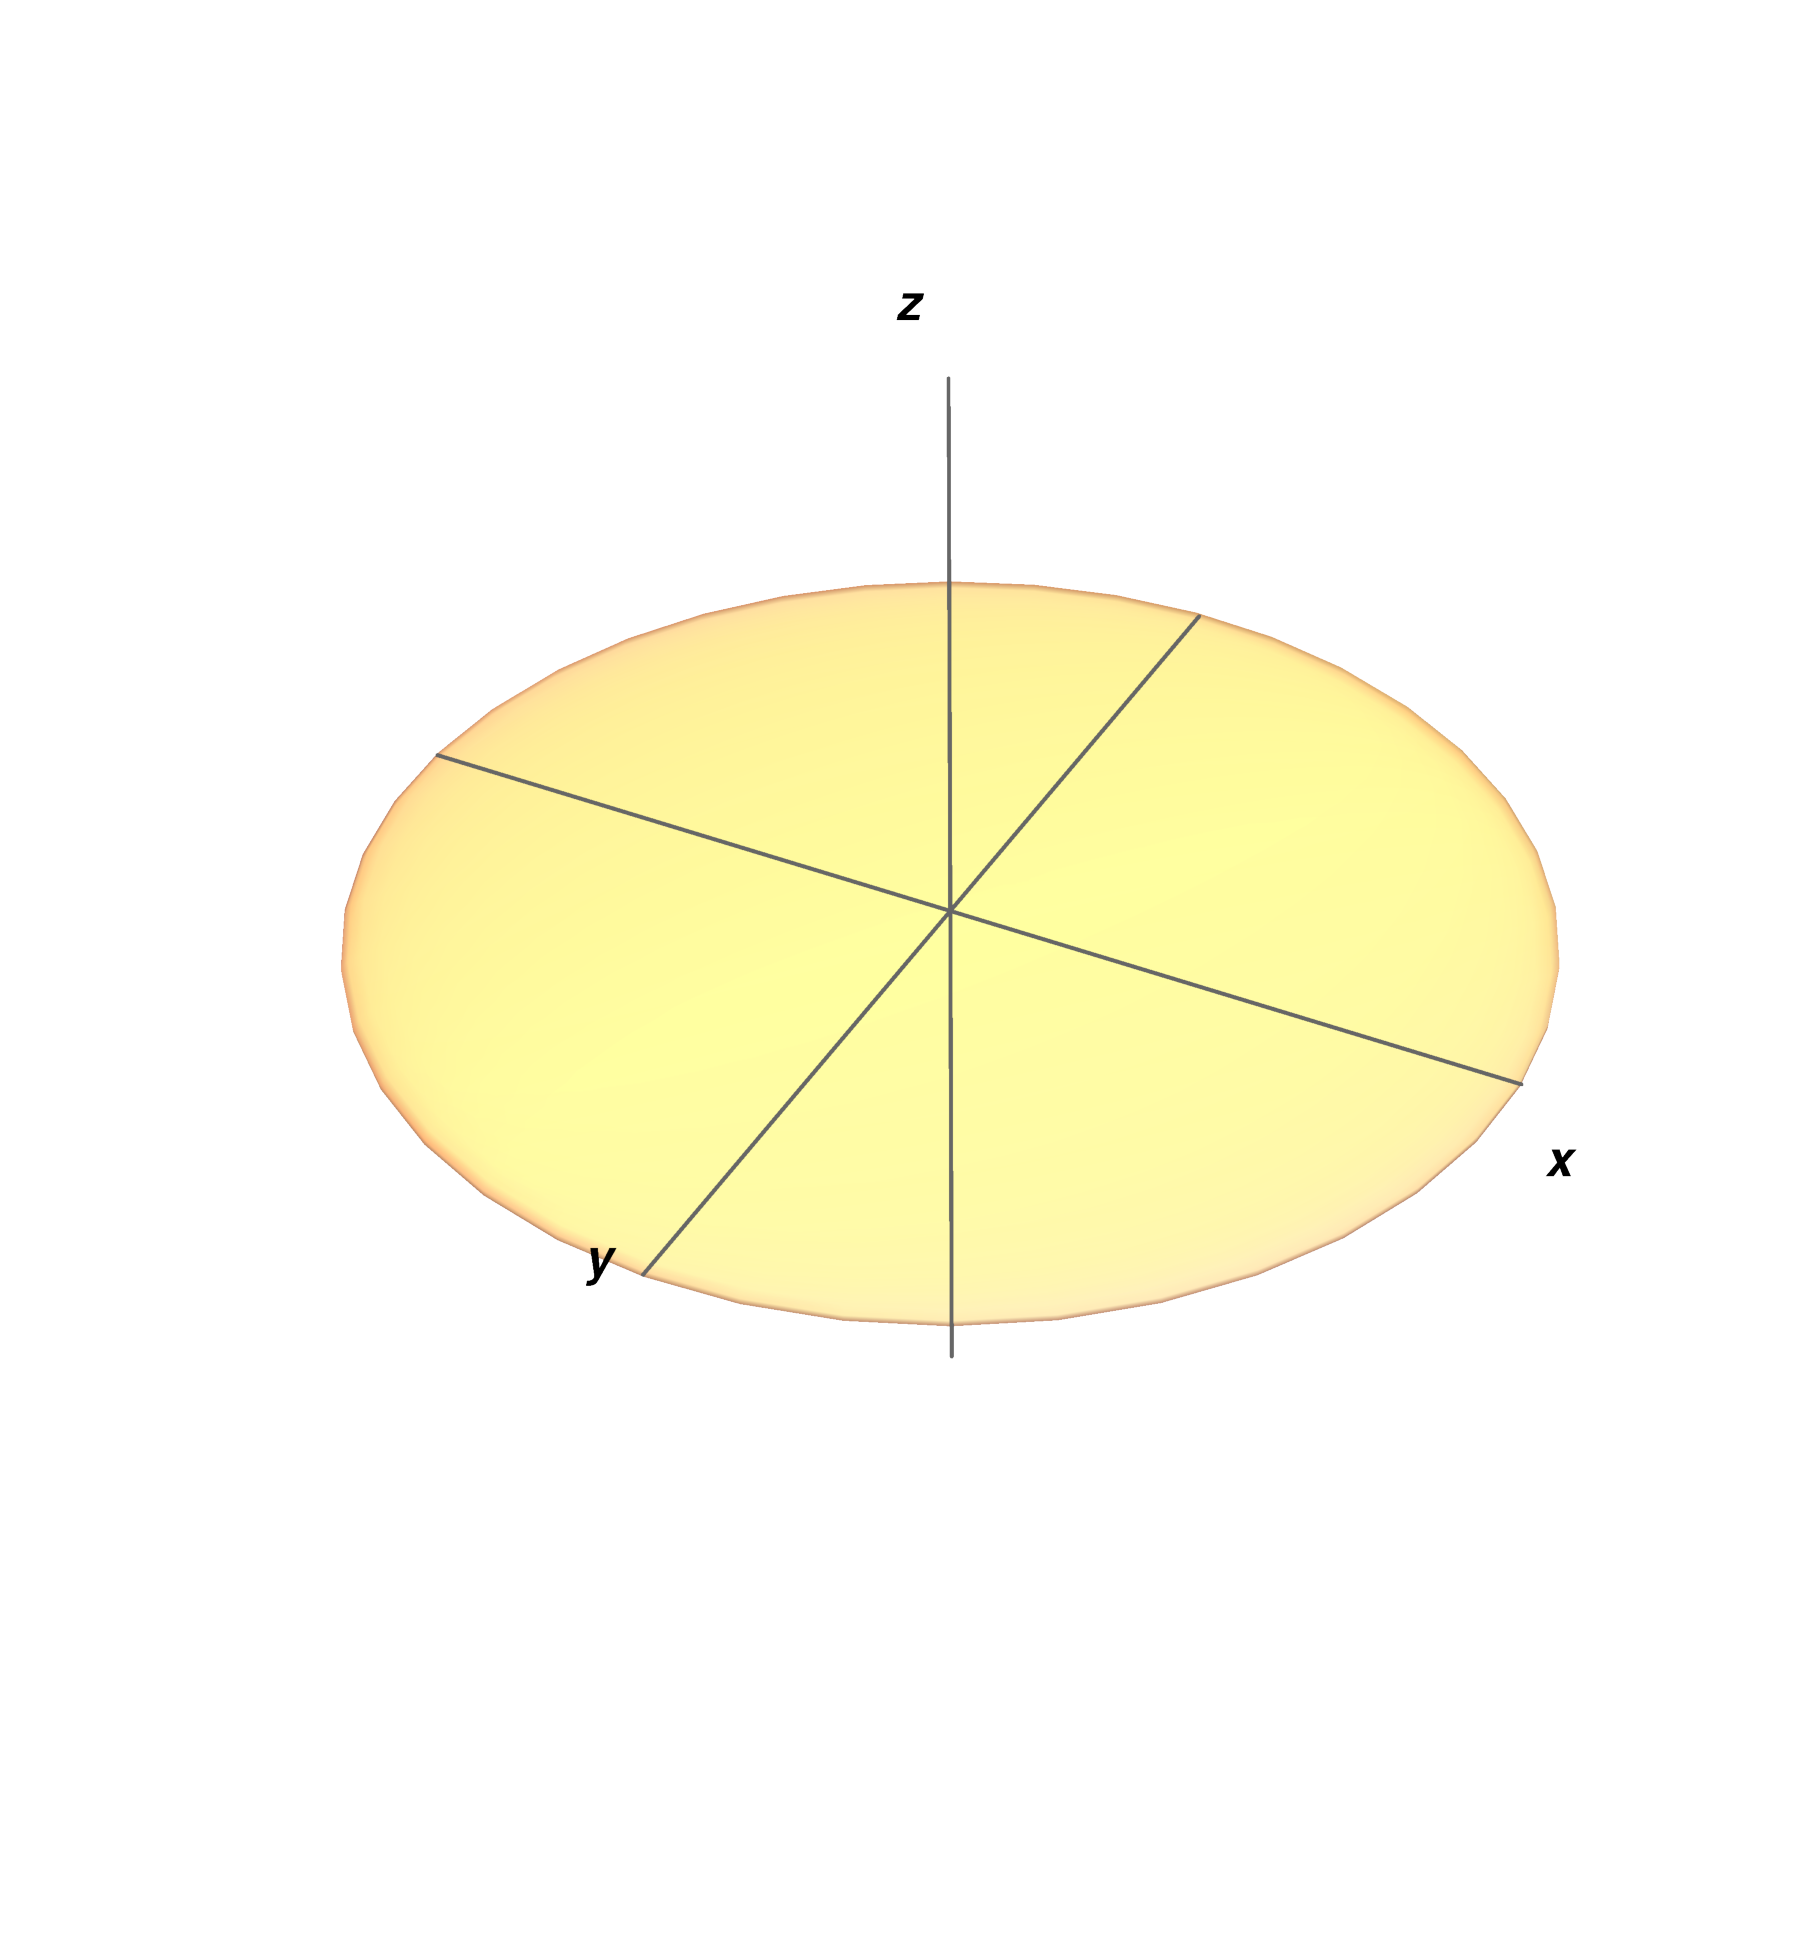
\includegraphics[height=0.5\textheight]{img-congreso/DiskXY.pdf}
			\end{figure}
		\end{column}
	\end{columns}	
	\begin{align*}
		\colorbox{Red}{$\qty(r_x,r_y,r_z) 
		\longrightarrow \qty(r_x,r_y,0)$}
	\end{align*}
	}
	
	\only<4>{
	Deformar la bola de Bloch en una línea:
	\begin{columns}
		\begin{column}{0.48\linewidth}
			\begin{figure}
				\centering
				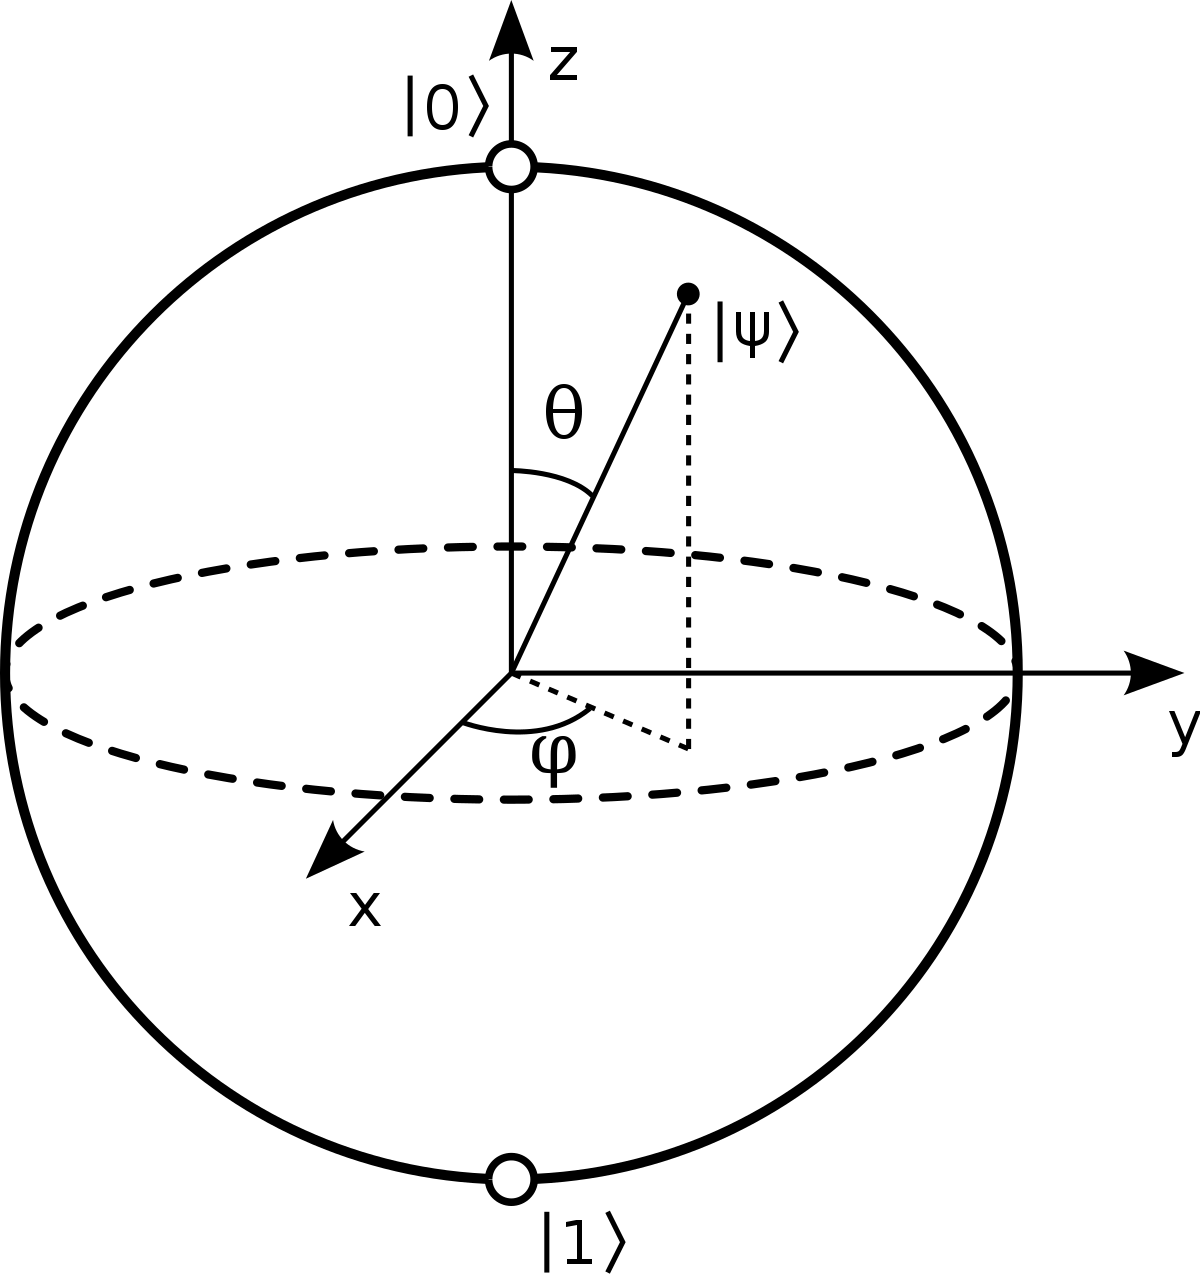
\includegraphics[height=0.5\textheight]{blochSphere.pdf}
			\end{figure}
		\end{column}
		\begin{column}{0.05\linewidth}
			\centering	
			\huge
			\colorbox{YellowGreen}{$\longrightarrow$}
		\end{column}
		\begin{column}{0.5\linewidth}
			\begin{figure}
				\centering
				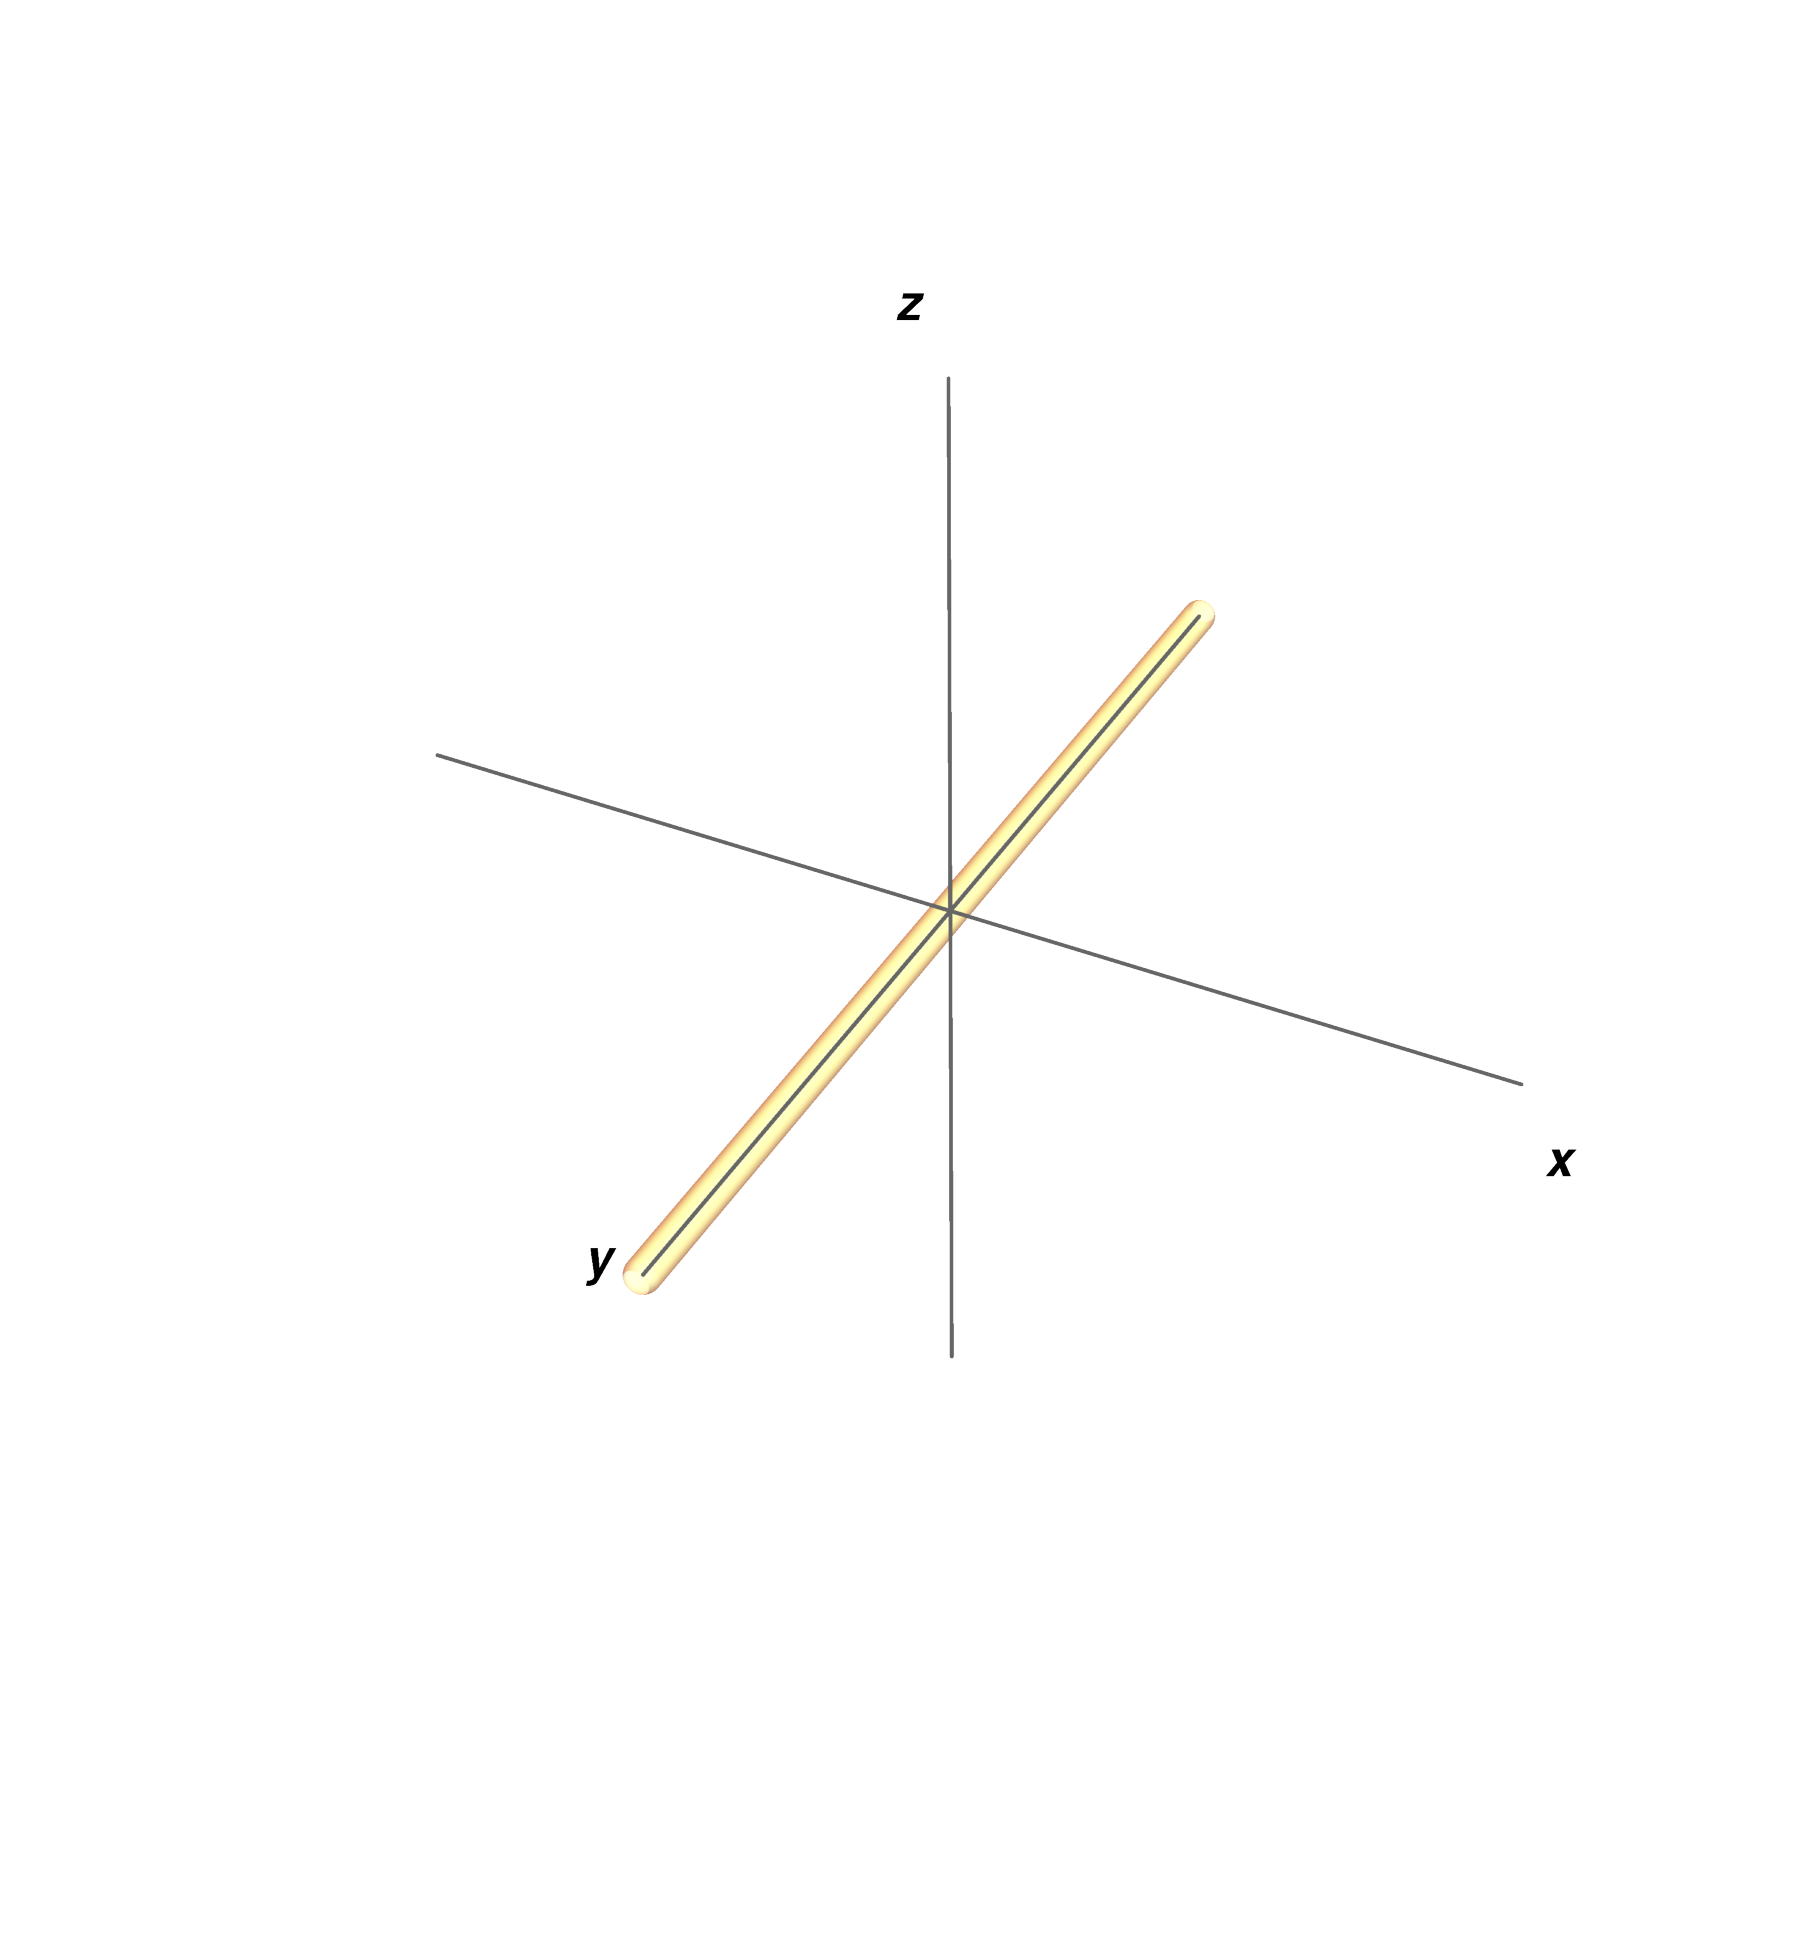
\includegraphics[height=0.5\textheight]{img-congreso/lineY.pdf}
			\end{figure}
		\end{column}
	\end{columns}	
	\begin{align*}
		\colorbox{YellowGreen}{$\qty(r_x,r_y,r_z) 
		\longrightarrow \qty(0,r_y,0)$}
	\end{align*}
	}
	
	\only<5>{
	Deformar la bola de Bloch en un punto en el origen:
	\begin{columns}
		\begin{column}{0.48\linewidth}
			\begin{figure}
				\centering
				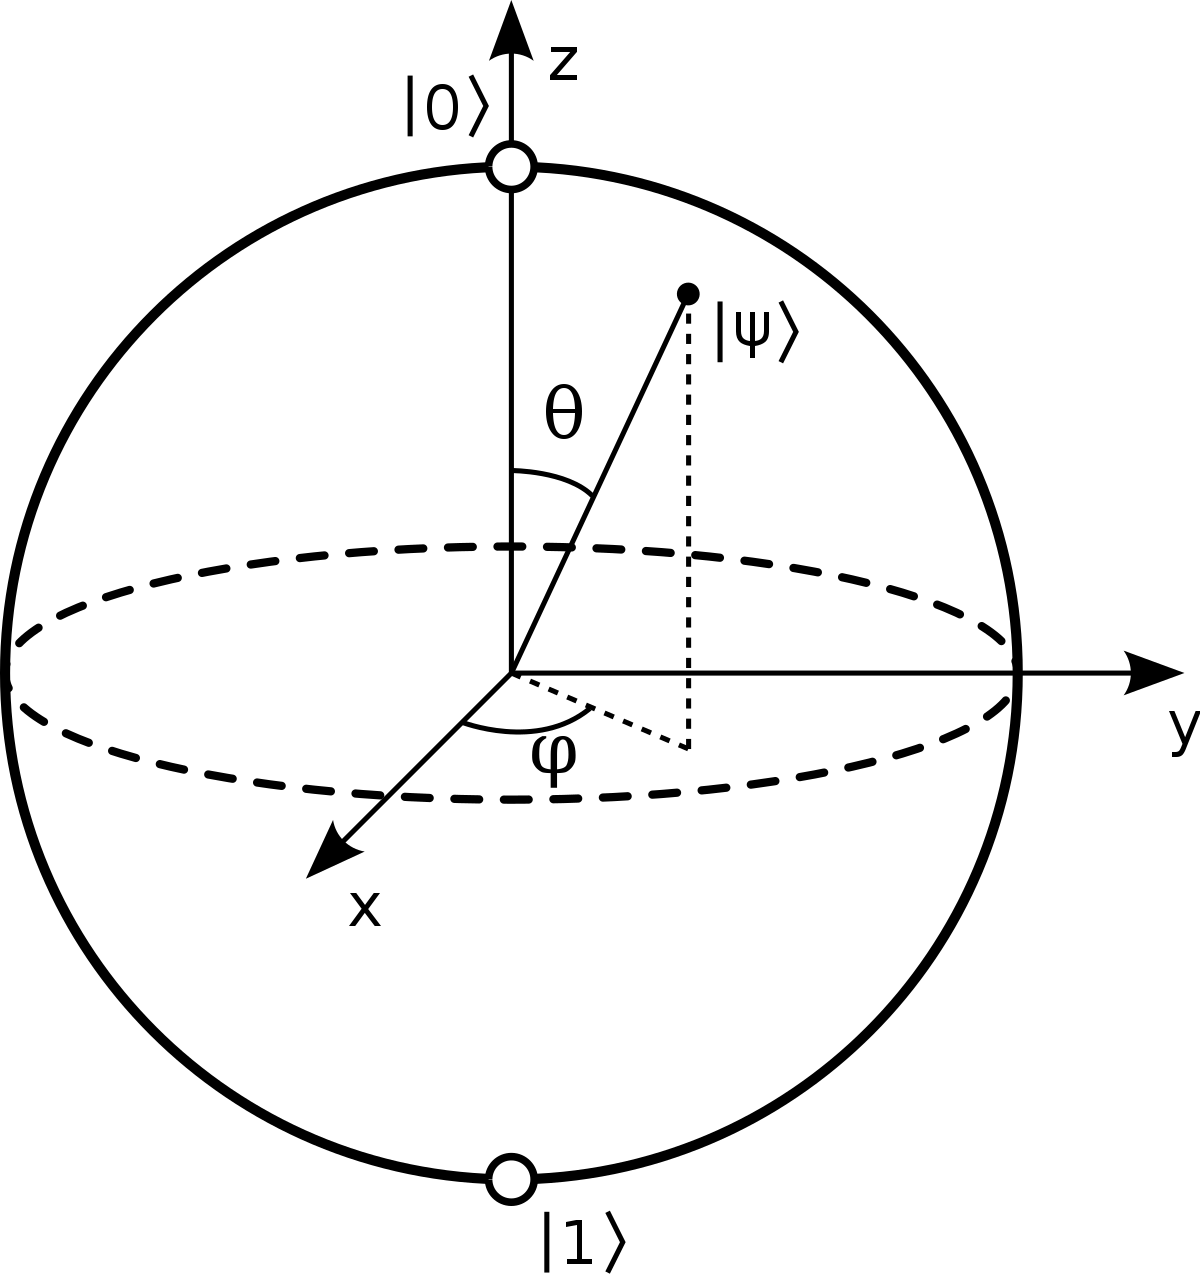
\includegraphics[height=0.5\textheight]{blochSphere.pdf}
			\end{figure}
		\end{column}
		\begin{column}{0.05\linewidth}
			\centering	
			\huge
			\colorbox{YellowGreen}{$\longrightarrow$}
		\end{column}
		\begin{column}{0.5\linewidth}
			\begin{figure}
				\centering
				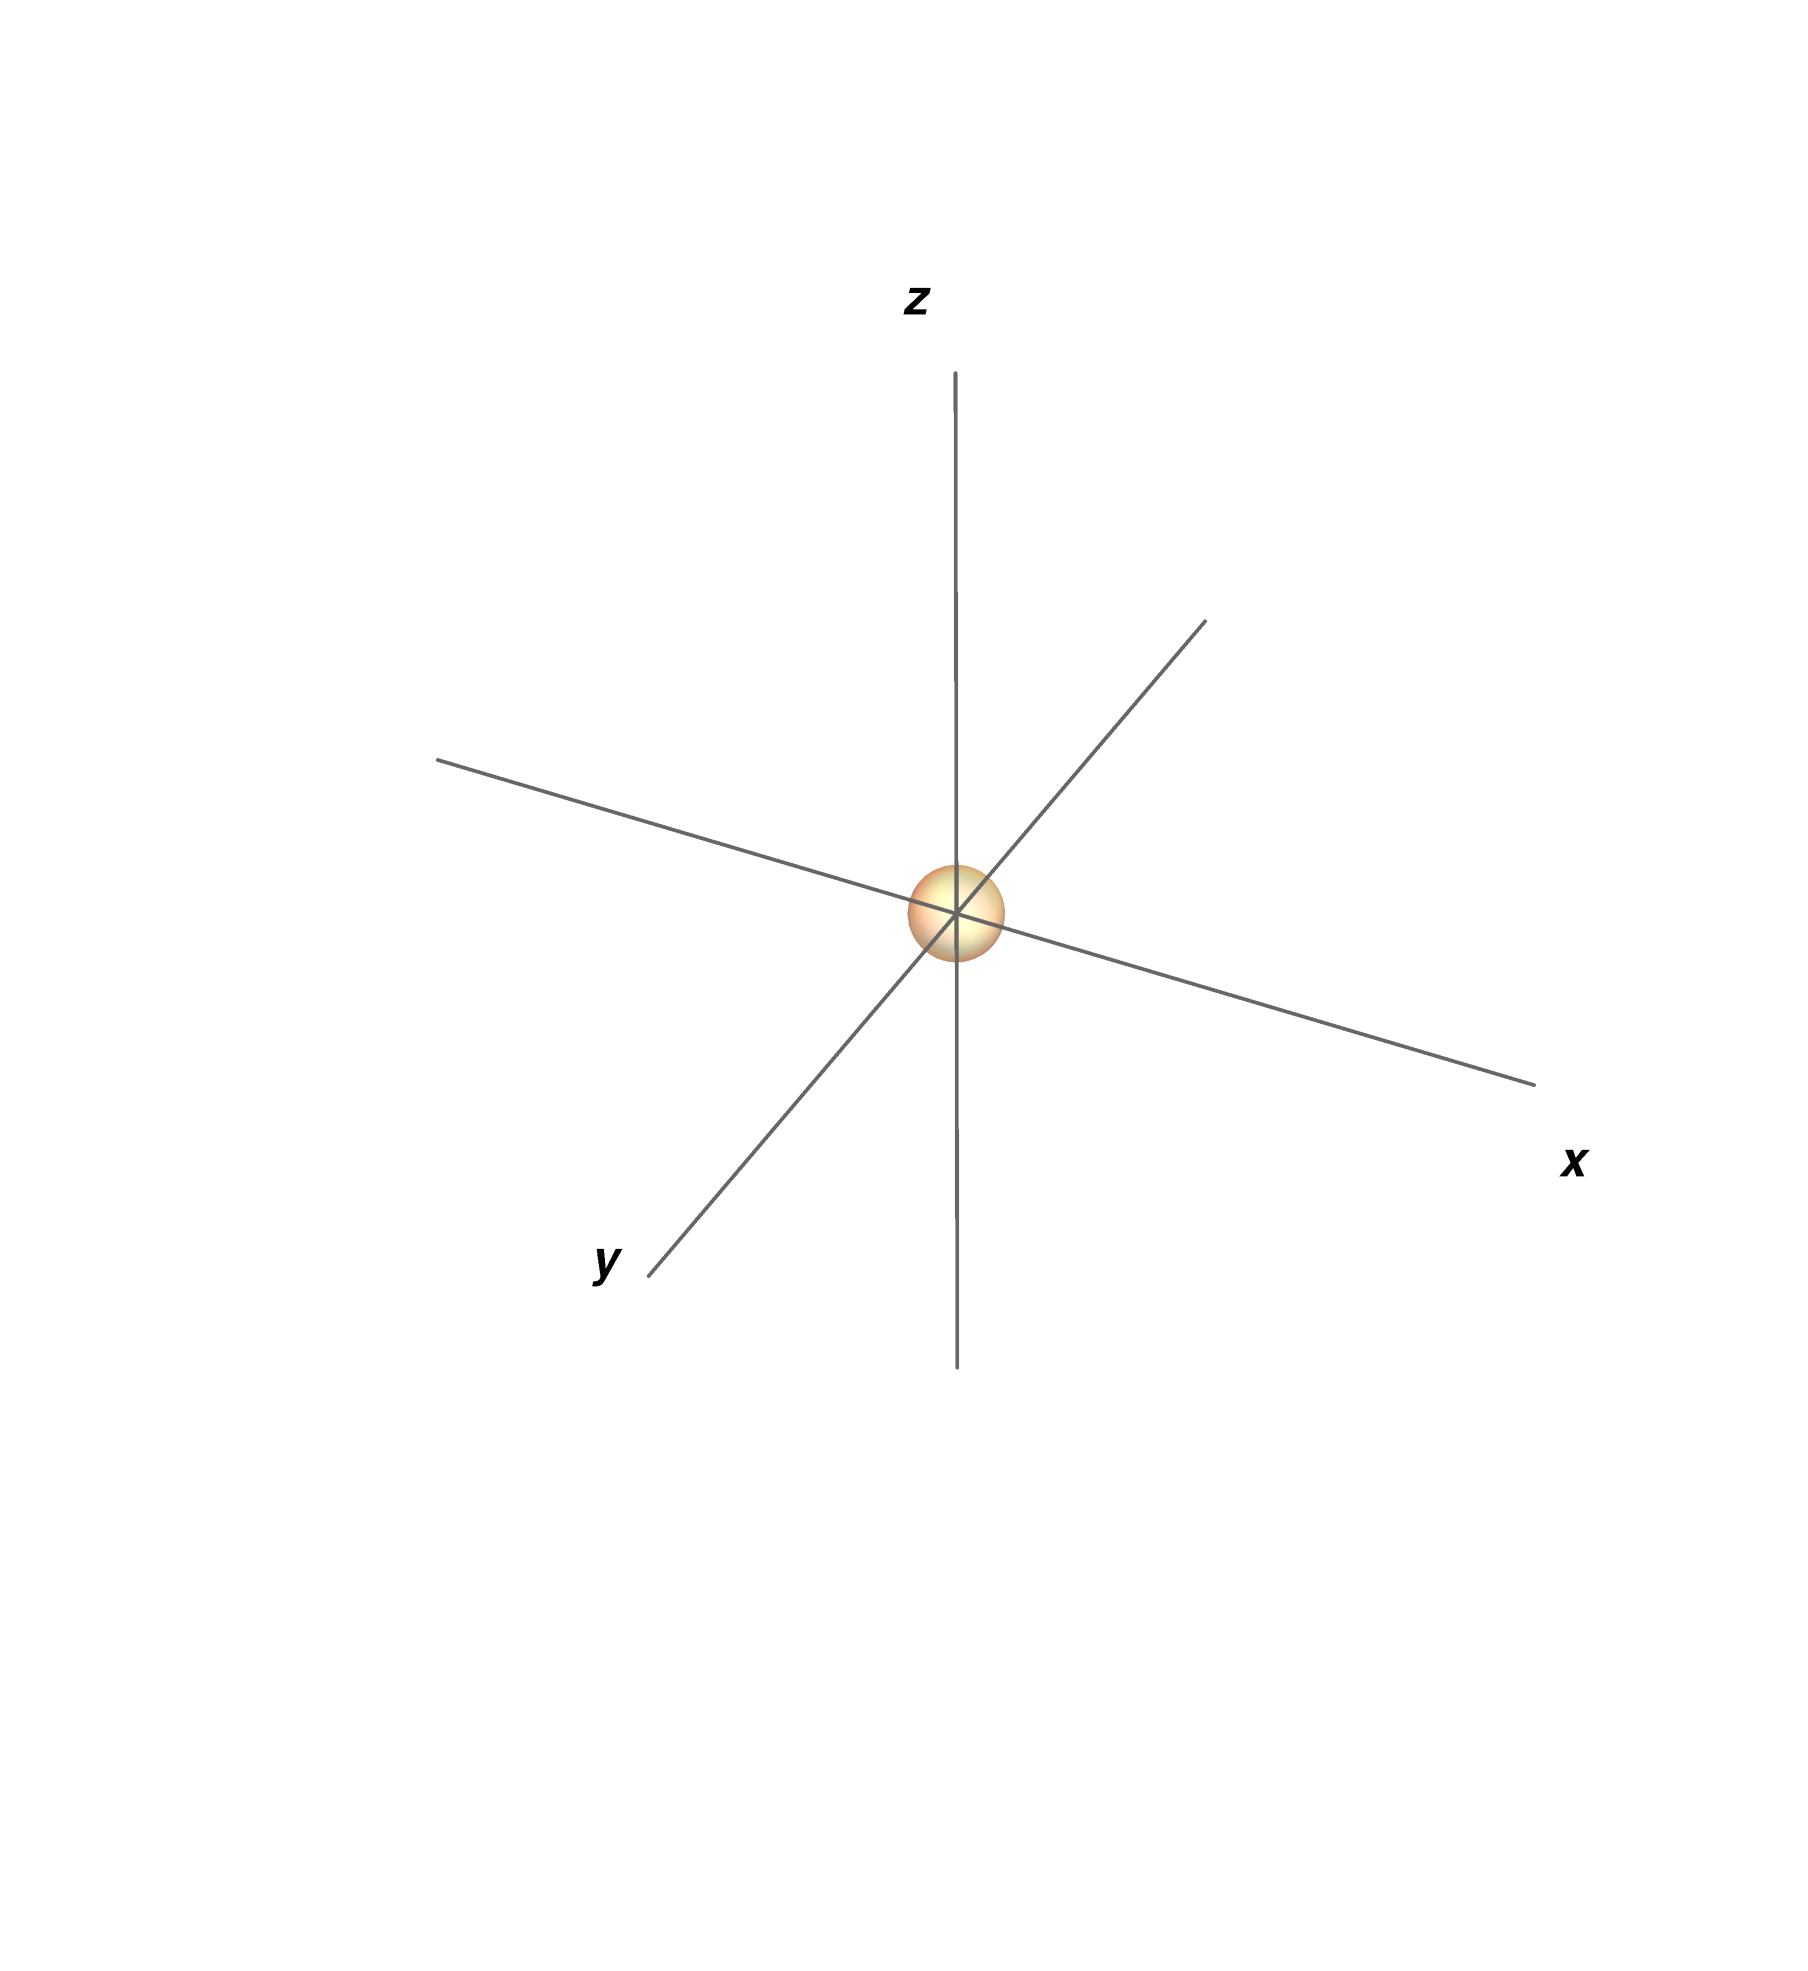
\includegraphics[height=0.48\textheight]{img-congreso/origin.pdf}
			\end{figure}
		\end{column}
	\end{columns}	
	\begin{align*}
		\colorbox{YellowGreen}{$\qty(r_x,r_y,r_z) 
		\longrightarrow \qty(0,0,0)$}
	\end{align*}
	}

\end{frame}


\begin{frame}{En conclusión, para 1 qubit}
	\begin{itemize}[label=$\textcolor{Blue}{\blacktriangleright}$]
		\item son canales cuánticos los mapeos que mantienen
						invariantes 1, 2 y 4 componentes de $\rho$,
		\begin{align*}
			\rho = \frac{\alert{r_0}\mathbb{1} + \alert{\mathbf{r_x}}\sigma _x 
			+ \alert{\mathbf{r_y}}\sigma _y	+ \alert{\mathbf{r_z}}\sigma _z}{2}, 
			\hspace{20pt} r_0 = 1.
		\end{align*}					
	\end{itemize}
	
	
\end{frame}




\begin{frame}
	\begin{itemize}[label=$\textcolor{Blue}{\blacktriangleright}$]
		\item<1-> Vamos a adoptar una nueva representación de $\rho$ de 1 qubit 
		\begin{figure}
			\centering
			\begin{tikzpicture}
				\node[anchor=north,inner sep=0] at (0,1.1) {$\rho =$};
				\node[anchor=north,inner sep=0] at (0.7,1.8) {
				
\includegraphics[height=1.5cm]{img-congreso/tablero-1q.pdf}};
				\node[anchor=north,inner sep=0] at (1,1) {.};
			\end{tikzpicture}
		\end{figure}
		\item<2-> En esta nueva representación los canales cuánticos de 1 qubit
		son aquellos cuyas matrices de densidad resultantes son
		\vspace{0.7cm}
		\begin{center}
			\begin{tikzpicture}
%					\draw[thick, ->] (-1,1.5) node[anchor=east]
%					{\includegraphics[width=5mm]
%					{img-congreso/tablero-1q.pdf}} -- (-0.05,1.5);
%					\draw[thick] (0,0) rectangle (2,3);
%					\node[anchor=north,inner sep=0] at (1,1.8) {\Huge $\Phi$};
%					\draw[thick, ->] (2.05,1.5) -- (3,1.5) 
					\node[anchor=north, inner sep=0] at (0,0) 
					{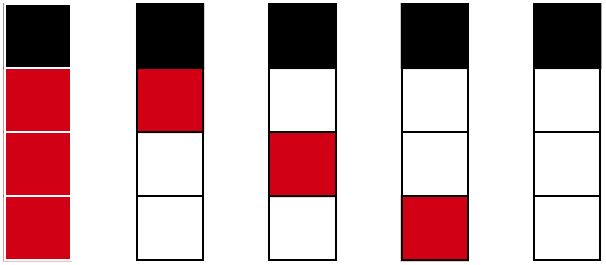
\includegraphics[width=4.2cm]{img-congreso/1q-CCs.png}};
					\node[anchor=north,inner sep=0] at (2.5,-1) {.};
			\end{tikzpicture}
		\end{center}
	\end{itemize}
\end{frame}



\subsection{2 qubits}
\begin{frame}{2 qubits}
	La matriz de densidad de 2 qubits 
	\begin{align*}
		\rho = \frac{1}{4} \sum _{i,j=0}^3 r_{ij} \sigma _i \otimes \sigma _j,
	\end{align*}\vfill \pause

	traducido a la representación de cuadritos pintados:
	\begin{figure}[H]
		\centering
	  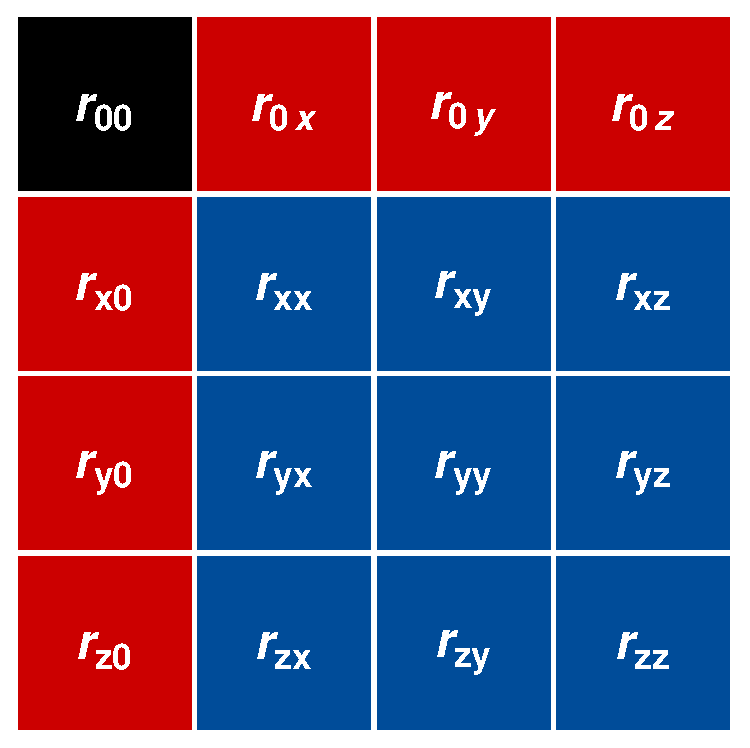
\includegraphics[width=3.2cm]{img-congreso/rho2q(2)}
	\end{figure}
\end{frame}



\begin{frame}
	Un mapeo en el que estamos interesados es
	\begin{center}
	\begin{tikzpicture}
			\draw[thick, ->] (-1,1.5) node[anchor=east] {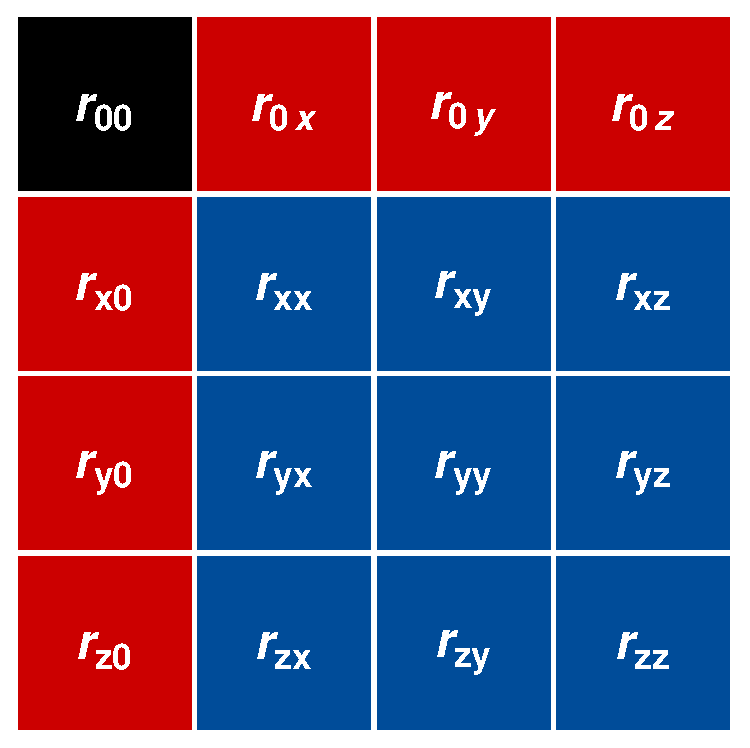
\includegraphics[width=2.5cm]{img-congreso/rho2q(2)}} -- (-0.05,1.5);
			\draw[thick] (0,0) rectangle (2,3);
			\node[anchor=north,inner sep=0] at (1,1.8) {\Huge $\Phi$};
			\draw[thick, ->] (2.05,1.5) -- (3,1.5) node[anchor=west] {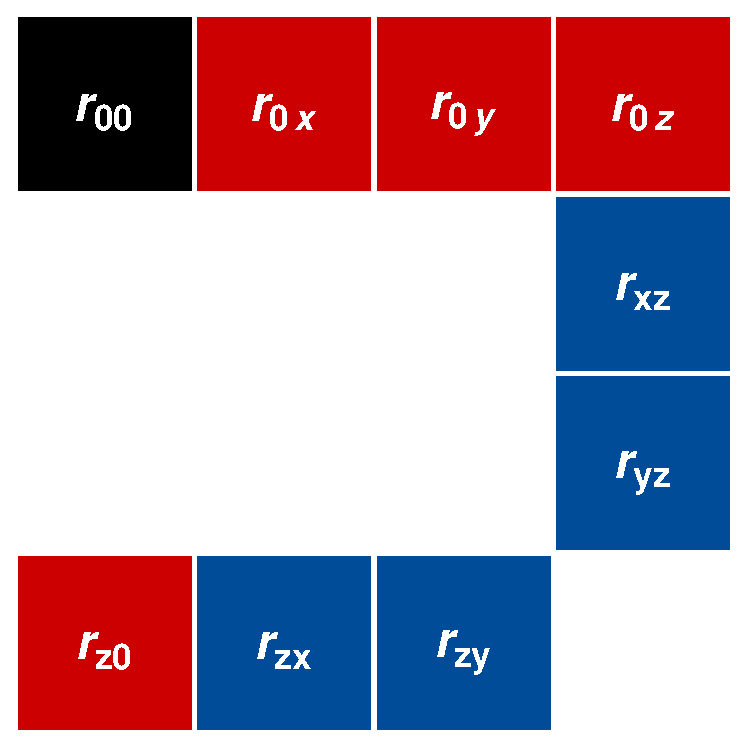
\includegraphics[width=2.5cm]{img-congreso/ex-2q-map}};
	\end{tikzpicture}
	\end{center}\pause
	
	\begin{itemize}[label=$\textcolor{Blue}{\blacktriangleright}$]
		\item<2-> 15 componentes que se pueden dejar invariantes o borrar
		\item<3-> $2^{15}$ (32,768) mapeos posibles
	\end{itemize}
\end{frame}

\begin{frame}
	\begin{itemize}[label=$\textcolor{Blue}{\blacktriangleright}$]
		\item 67 son canales cuánticos.
	\end{itemize}
	\begin{figure}
		\centering 
		
\includegraphics[height=0.6\textheight]{img-congreso/surprised}
	\end{figure}
\end{frame}




\begin{frame}%{\scriptsize{Resultados 2 qubits}}
\scriptsize
\begin{columns}
		\begin{column}{.49\textwidth}
			\begin{figure}
			$\boldsymbol{\text{C}^1}:$ \hfill $\mathtt{1}$ \newline
			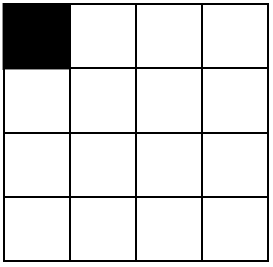
\includegraphics[width=7mm]{img-congreso/C16.png} \hfill \hfill
			\vspace{1mm}
			\hrule
			\vspace{1mm}
			$\boldsymbol{\text{C}_1^2}:$ \hfill $\mathtt{15}$ \newline
			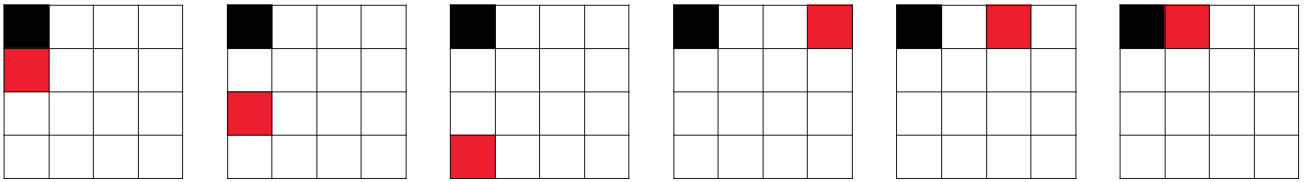
\includegraphics[width=\textwidth]{img-congreso/C12.png} \newline
			$\boldsymbol{\text{C}_2^2}:$ \hfill \hfill \newline
			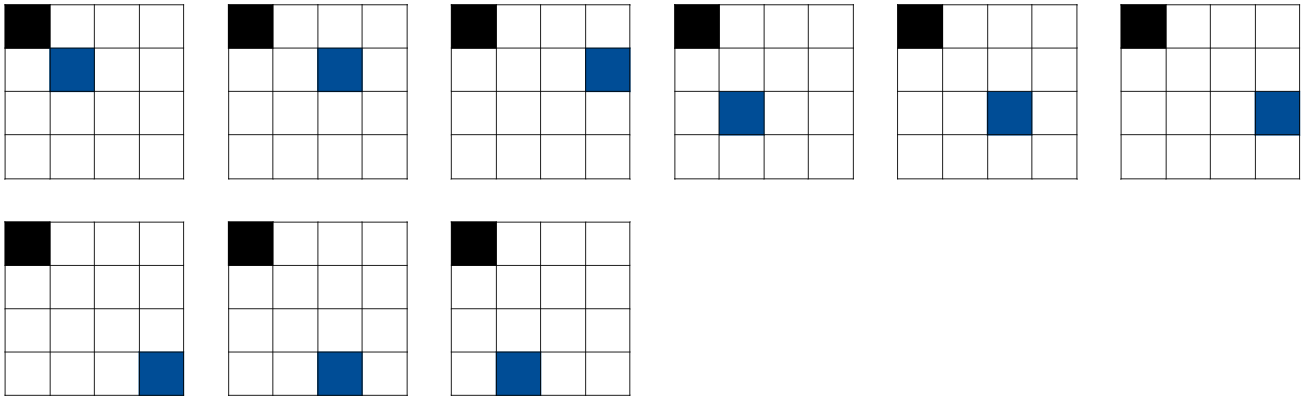
\includegraphics[width=\textwidth]{img-congreso/C22.png} \hfill \hfill
			\vspace{1mm}
			\hrule
			\vspace{1mm}
			$\boldsymbol{\text{C}_1^4}:$ \hfill $\mathtt{35}$ \newline
			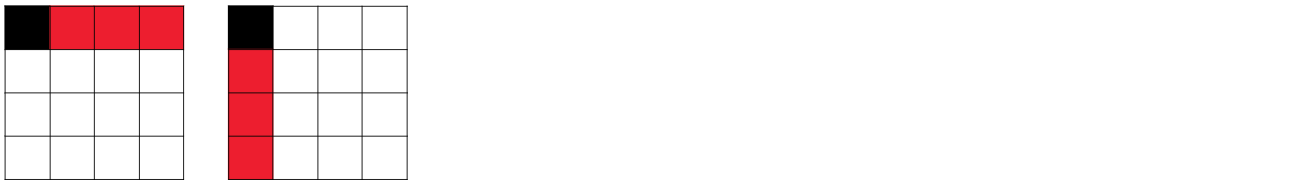
\includegraphics[width=\textwidth]{img-congreso/C14.png} \newline
			$\boldsymbol{\text{C}_2^4}:$ \hfill \hfill  \newline
			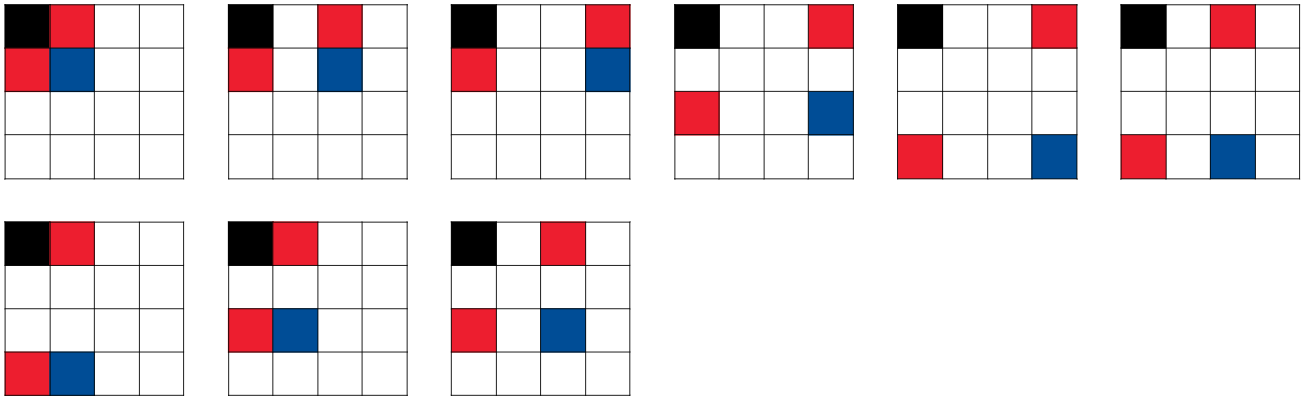
\includegraphics[width=\textwidth]{img-congreso/C24.png} \newline
		\end{figure}
	\end{column}
	\begin{column}{.49\textwidth}
		\begin{figure}
			$\boldsymbol{\text{C}_3^4}:$ \hfill \hfill \newline
			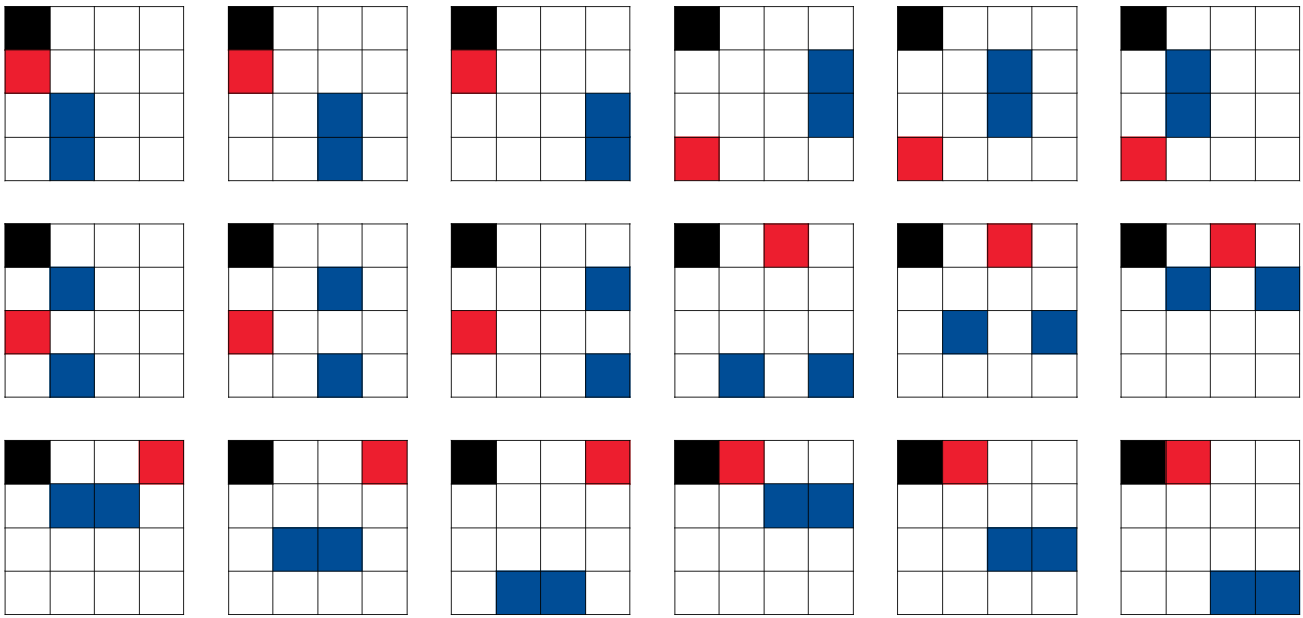
\includegraphics[width=\textwidth]{img-congreso/C34.png} \newline
			$\boldsymbol{\text{C}_4^4}:$ \hfill \hfill \newline
			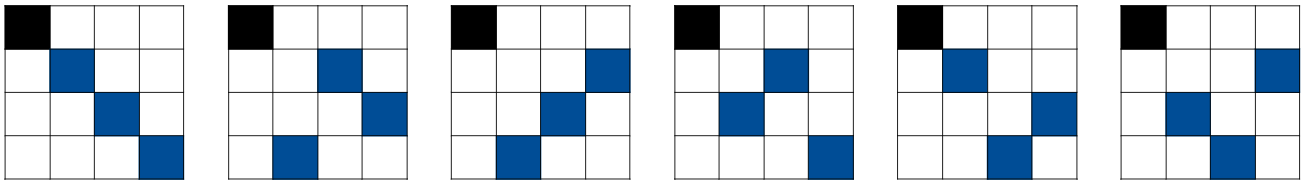
\includegraphics[width=\textwidth]{img-congreso/C44.png}
			\hrule
			\vspace{1mm}
			$\boldsymbol{\text{C}_1^8}:$ \hfill $\mathtt{15}$ \newline
			\includegraphics[width=\textwidth]{img-congreso/C18.png} \newline
			$\boldsymbol{\text{C}_1^8}:$ \hfill \hfill \newline
			\includegraphics[width=\textwidth]{img-congreso/C28.png} 
			\hrule
			$\boldsymbol{\text{C}^{16}}:$ \hfill $\mathtt{1}$ \newline
			\includegraphics[width=7mm]{img-congreso/C0.png} \hfill \hfill
		\end{figure}
		\vfill
	\end{column}
\end{columns}
	\vfill
\end{frame}




%\begin{frame}
%	\textbf{2 componentes invariantes}
%	\begin{itemize}[label=$\textcolor{Blue}{\blacktriangleright}$]
%		\item	Mapeos posibles = $\mathcal{C}(15,1)=\colorbox{LimeGreen}{15}$\hfill
%				canales cuánticos = \colorbox{LimeGreen}{15}
%	\end{itemize}	
%	\begin{figure}[H]
%	\centering
%	  \begin{minipage}{0.9\textwidth}
%	  	$\boldsymbol{C_1^2}:$ 
%	  	\begin{center}
%	  		\includegraphics[width=.9\textwidth]{img-congreso/C12.png}
%	  	\end{center}
%	  	Se mantiene invariante 1 componente de 1 qubit y se borra
%	  	el resto.
%	  \end{minipage}\vspace*{.15cm}
%	  \begin{minipage}{0.9\textwidth}
%	  	 $C_2^2$:
%			\begin{center}
%				\includegraphics[width=.9\textwidth]{img-congreso/C22.png}
%			\end{center}
%			Se borra todo excepto una correlación del sistema.
%	  \end{minipage}
%	\end{figure}
%
%\end{frame}
%
%
%
%\begin{frame}
%	\textbf{4 componentes invariantes}
%	\begin{itemize}[label=$\textcolor{Blue}{\blacktriangleright}$]
%		\item	Mapeos posibles = $\mathcal{C}(15,3)=\colorbox{BurntOrange}{455}$\hfill
%					canales cuánticos = \colorbox{LimeGreen}{35}
%	\end{itemize}	
%	\only<1>{
%	\begin{figure}[H]
%	\centering
%	  \begin{minipage}{0.48\textwidth}
%	  	$C_1^4$:
%	  	\begin{center}
%	    	\includegraphics[width=\textwidth]{img-congreso/C14.png}
%	  	\end{center}
%	  	\vspace{0.8cm}
%	  	\footnotesize Un qubit se deja invariante, se borra el resto.
%	  \end{minipage}\hfill
%	  \begin{minipage}{0.48\textwidth}
%	  	$C_2^4$:
%	  	\begin{center}
%	  		\includegraphics[width=\textwidth]{img-congreso/C24.png}
%	  	\end{center}
%	  	\footnotesize Se mantienene la componente $i$ de un qubit y la $j$ del otro,
%	  	además la correlación $ij$.
%	  \end{minipage}\vfill
%	  
%	  \begin{minipage}{0.48\textwidth}
%	  	$C_3^4$:
%	  	\begin{center}
%	  		\includegraphics[width=\textwidth]{img-congreso/C34.png}
%	  	\end{center}
%	  	\footnotesize ... ¿?
%	  \end{minipage}\hfill
%	  \begin{minipage}{0.48\textwidth}
%			$C_4^4$:
%			\begin{center}
%				\includegraphics[width=\textwidth]{img-congreso/C44.png}
%			\end{center}
%			\footnotesize Sólo se mantienen invariantes correlaciones del sistema.
%			%\vspace{45pt}
%	  \end{minipage}
%	\end{figure}
%	}	
%\end{frame}
%
%\begin{frame}
%	\textbf{4 componentes invariantes:}	\alert{¿cómo cuáles no son posibles?}
%	\begin{figure}
%		\centering
%		\includegraphics[width=0.8\textwidth]{img-congreso/2q-C4-notCC.png}
%	\end{figure}	
%	\begin{itemize}[label=$\textcolor{Blue}{\blacktriangleright}$]
%		\item No sólo importa el número de componentes invariantes
%		sino también \textbf{cuáles} componentes de $\rho$ se mantienen 
%		invariantes.
%	\end{itemize}
%\end{frame}
%
%
%
%\begin{frame}
%	\textbf{8 componentes invariantes}
%	\begin{itemize}[label=$\textcolor{Blue}{\blacktriangleright}$]
%		\item	Mapeos posibles: $\mathcal{C}(15,7)=\colorbox{BurntOrange}{6435}$\hfill
%					canales cuánticos: \colorbox{LimeGreen}{15}
%	\end{itemize}	
%	
%	\begin{figure}[H]
%	\centering
%	  \begin{minipage}{0.7\textwidth}
%	  	$C_1^8$:
%	  	\begin{center}
%	  		\includegraphics[width=\textwidth]{img-congreso/C18.png}
%	  	\end{center}
%	  \end{minipage}\vfill
%	  \begin{minipage}{0.7\textwidth}
%	  	$C_2^8$:
%	  	\begin{center}
%	  		\includegraphics[width=\textwidth]{img-congreso/C28.png}
%	  	\end{center}
%	  \end{minipage}
%	\end{figure}
%	
%	\begin{itemize}[label=$\textcolor{Blue}{\blacktriangleright}$]
%		\item También hay 15 canales cuánticos que mantienen invariantes 2 
%					componentes de $\rho$, ¿existirá algún tipo de relación entre 
%					ambos subconjuntos de canales de 2 qubits?
%	\end{itemize}
%\end{frame}
%
%
%
%\begin{frame}
%	\large{\textbf{16 componentes invariantes}}
%	\begin{itemize}[label=$\textcolor{Blue}{\blacktriangleright}$]
%		\item Mapeos posibles = $\mathcal{C}(15,15)=\colorbox{LimeGreen}{1}$\hfill
%					canales cuánticos: \colorbox{LimeGreen}{1} 			
%	\end{itemize}	
%	\normalsize
%	\begin{figure}
%		\includegraphics[width=2cm]{img-congreso/C0.png}
%	\end{figure}
%	El estado del sistema de qubits se deja igual, este es el canal identidad. 
%\end{frame}




\begin{frame}{\Large ¿Qué aprendimos de 2 qubits?}
%	\only<1->{\textbf{¿Qué aprendimos de 2 qubits?}}
	
	\begin{itemize}[label=$\textcolor{Blue}{\blacktriangleright}$]
		\item<2-> El número de componentes invariantes que dejan estos canales 
							cuánticos debe ser una potencia de 2,
		\only<2>{\vspace{1cm}}
			\only<3->
			{
			\vspace{1mm}
			\scriptsize{
			\begin{center}
			\begin{tabular}{r|c|c|c|c|c}
			\textbf{no. de comp. invariantes} & $2^0$ & $2^1$ & $2^2$ & $2^3$ & $2^4$ \\ 
			\hline 
			\textbf{no. de canales cuánticos} & 1 & 15 & 35 & 15 & 1 \\ 
			\end{tabular} 
			\end{center}
			}}
%		\only<3>{
%				\begin{figure}
%					\centering
%					\includegraphics[width=4cm]{img-congreso/obey.png}
%					\newline
%					\hfill \colorbox{green}{válido} \hspace{.5cm} 
%					\colorbox{red}{inválido} \hspace{.15\textwidth}
%				\end{figure}
%		}				
					
					%(sobre cada uno de 
					%los vectores de Bloch deben haber acciones válidas de 1 qubit.)
%		\only<5>{
%				\begin{figure}
%					\centering
%					\includegraphics[width=0.5\textwidth]{img-congreso/power-of-2.png}
%					\newline
%					\hspace{1.5cm} \colorbox{green}{válido} \hspace*{1.2cm} 
%					\colorbox{red}{no válido} \hspace{1cm}
%				\end{figure}
%		}
		\item<4-> Estos canales cuánticos son equivalentes ante intercambio de 
							qubits (transposiciones en los tableros).
					
		\item<5-> También son equivalentes ante permutaciones de las 
							componentes $x$, $y$ y $z$ de cada partícula 
							(permutación de las filas o columnas 1-3).
		\item<6-> La acción individual de un canal cuántico de 2 qubits sobre 
							cada partícula del sistema debe ser un canal cuántico de 1 qubit.	
%		\only<7>{
%				\begin{figure}
%					\centering
%					\includegraphics[width=2.1cm]{img-congreso/transposition.png}\hfill					
%					\includegraphics[width=2.1cm]{img-congreso/1.png}\hfill
%					\includegraphics[width=2.1cm]{img-congreso/2.png}\hfill
%					\includegraphics[width=2.1cm]{img-congreso/3.png}\newline
%					\footnotesize{
%					\hspace*{1cm} cambio q1$\rightarrow$q2 \hspace*{2mm} 
%					$x_2,y_2,z_2\rightarrow					z_2,x_2,y_2$
%					\hspace*{2mm} $z_2,x_2,y_2 \rightarrow y_2,z_2,x_2$ \hfill}
%				\end{figure}
%				}					
	\end{itemize}
\end{frame}



\subsection{3 qubits}
\begin{frame}{3 qubits}
	La matriz de densidad de 3 qubits
	\begin{align*}
		\rho = \frac{1}{8} \sum _{i,j,k=0}^3 r_{ijk} \sigma _i \otimes \sigma _j
		\otimes \sigma _k, \hspace{15pt}
		%\text{(¡63 }r_{ijk}\text{ distintas!)};
	\end{align*}\pause
	traducido a la descripción de \textit{cubos pintados}
	\begin{figure}
		\includegraphics[height=0.4\textheight]{img-congreso/rho-3q}
	\end{figure}
	%$2^{63}\thicksim 9\times 10^{18}$ mapeos posibles. \vfill
	
	% Agregar a notas de las diapositivas
	%Reducir el análisis numérico sólo a los mapeos que dejan 8 componentes 
	%invariantes	representaría diagonalizar $\thicksim$ 550 millones de 
	%matrices de dimensión $64\times 64$.
\end{frame}


\begin{frame}{Resultados 3 qubits\footnote{Numéricamente, hemos podido analizar
los mapeos que dejan hasta 4 componentes invariantes en $\rho$}}\pause
	Resultados que entendemos de resultados previos:
	\begin{figure}
		\includegraphics[width=.2\textwidth]{img-congreso/3q-4c-04} \hfill
		\includegraphics[width=.2\textwidth]{img-congreso/3q-4c-01} \hfill
		\includegraphics[width=.2\textwidth]{img-congreso/3q-4c-03} \hfill
		\includegraphics[width=.2\textwidth]{img-congreso/3q-4c-02} \hfill
	\end{figure}\pause
	Resultados que no entendemos (\textbf{¿aún?})	de resultados previos:
	\begin{figure}
		\includegraphics[width=.2\textwidth]{img-congreso/3q-4c-1} \hfill
		\includegraphics[width=.2\textwidth]{img-congreso/3q-4c-2} \hfill
		\includegraphics[width=.2\textwidth]{img-congreso/3q-4c-3} \hfill
 		\includegraphics[width=.2\textwidth]{img-congreso/3q-4c-4} \hfill
	\end{figure}
\end{frame}


\subsection{n qubits}
%\begin{frame}{n qubits}
%	La matriz de densidad de $n$ qubits es
%	\begin{align*}
%		\rho = \sum _{\vec{v}} \frac{\Tr \qty( \sigma _{v_1} \otimes 
%		\sigma _{v_2} \otimes \cdots \otimes \sigma _{v_n}\rho) \sigma _{v_1} 
%		\otimes \sigma _{v_2} \otimes \cdots \otimes \sigma _{v_n}}{2^n},
%	\end{align*}
%	donde la sumatoria va sobre los vectores $\vec{v}=\qty(v_1, v_2, \cdots, 
%	v_n)$ con entradas $v_i$ seleccionadas del conjunto $\{ 0,1,2,3\}$.\vfill
%	
%	Los coeficientes $\Tr \qty( \sigma _{v_1} \otimes \sigma _{v_2} \otimes 
%	\cdots \otimes \sigma _{v_n}\rho)$ son las componentes de $\rho$ que los
%	mapeos pueden dejar invariantes o borrar.
%\end{frame}

\begin{frame}{Características de los canales cuánticos de $n$ 
qubits}
	\begin{itemize}[label=$\textcolor{Blue}{\blacktriangleright}$]
	\item<2-> El número de componentes invariantes en $\rho$ son\newline
				potencias de 2. 
	\item<3-> \hfill
	\scriptsize{					
	\begin{center}
		\begin{tabular}{>{$n=}l<{$\hfill}*{12}{c}}
			1 &&&&&\colorbox{Apricot}{1}&3&\colorbox{Apricot}{1}&&&&5&\\
			2 &&&&\colorbox{CadetBlue}{1}&\colorbox{Cyan}{15}&35&\colorbox{Cyan}{15}&\colorbox{CadetBlue}{1}&&&67&\\
			3 &&&\colorbox{SpringGreen}{1}&\colorbox{RedOrange}{63}&\colorbox{Yellow}{561}&?&\colorbox{Yellow}{¿561?}&
				\colorbox{RedOrange}{¿63?}&\colorbox{SpringGreen}{1}&&?&\\		
%		
%			1 &&&&&\colorbox{Magenta}{1}&3&1&&&&&\\
%			2 &&&&1&\colorbox{Magenta}{15}&35&\colorbox{Magenta}{15}&1&&&&\\
%			3 &&&1&\colorbox{Orchid}{63}&\colorbox{Aquamarine}{561}&?&
%			\colorbox{Aquamarine}{¿561?}&\colorbox{Orchid}{¿63?}&1&&&\\
%			4 &&1&\colorbox{BrickRed}{255}&\colorbox{Yellow}{?}&
%			\colorbox{PineGreen}{?}&?&\colorbox{PineGreen}{?}
%			&\colorbox{Yellow}{?}&\colorbox{BrickRed}{255}&1&&\\
			\vdots &&\reflectbox{$\ddots$}&&&&$\vdots$&&&&$\ddots$&??
		\end{tabular}
	\end{center}
	} 
	\vspace{.2cm}	
	\onslide<4>{
	\normalsize
		\begin{figure}
			\includegraphics[width=4cm]{img-congreso/image}
		\end{figure}
	Hipótesis del arcoiris: correspondencia 1:1 entre canales que mantienen
	invariantes $2^k$ y $2^{n-k}$ componentes.}
	\end{itemize}
\end{frame}

\begin{frame}[noframenumbering]{Características de los canales cuánticos de $n$ 
qubits}
	\begin{itemize}[label=$\textcolor{Blue}{\blacktriangleright}$]
	\item<1-> Los canales son equivalentes ante intercambio de partículas y de
				permutación de las componentes individuales de cada qubit en el 
				sistema. 
	\item<2-> La acción de un canal sobre cualquier subsistema es otro canal.
	\end{itemize}

	\onslide<3>{
	\colorbox{Yellow}{Esto no es suficiente para caracterizar a estos 
	canales cuánticos.}
	}
\end{frame}
	


\section{Por hacer}

\begin{frame}{Dificultades}\pause

	\begin{itemize}[label=$\textcolor{Blue}{\blacktriangleright}$]
		\item \textbf{(numérica)}
		El número de mapeos posibles según el número de qubits crece como 
		$2^{4^n-1}$ (8, 32768, 9.2$\times 10^{18}$, 5.8$\times 10^{76}$, 
		7$\times 10^{187}$, $\ldots$).
		\pause
		
		\item Para $n>3$ no existe una representación geométrica útil que nos
		ayude a entender a los canales.
		
	\end{itemize}
\end{frame}

\begin{frame}{Preguntas por contestar}
	\begin{itemize}[label=$\textcolor{Blue}{\blacktriangleright}$]
		\item<2-> ¿Por qué estos canales siguen la regla de la potencia de 2 para el 
					número de componentes invariantes?
		\item<3-> ¿Es cierta la hipótesis del arcoiris? ¿Cuál es la correspondencia?
		\item<4-> ¿Existen transformaciones unitarias que conecten a elementos de
					distintas clases de equivalencia?
		\item<5-> ¿Existen reglas sencillas, equivalentes a la condición de completa
					positividad, que expliquen los patrones de los dibujos?
	\end{itemize}\vfill 
\end{frame}

\begin{frame}{Propuestas}
	\begin{itemize}[label=$\textcolor{Blue}{\blacktriangleright}$]
		\item<2-> Estudiar la representación en operadores de Krauss de estos 
					canales cuánticos. 
		\item<3-> Estudiar el espectro de Schmidt de la matriz de Choi asociada 
					a los canales cuánticos.
		\item<4-> Estudiar el isomorfismo de Jamiołkowski.
		\item<5-> Utilizar las reglas que entendemos de estos canales para reducir 
							los mapeos a analizar de forma numérica.
	\end{itemize}
\end{frame}


\begin{frame}{Trabajo futuro}
	\begin{itemize}[label=$\textcolor{Blue}{\blacktriangleright}$]
		\item<2-> Estudiar el efecto que tienen estos canales cuánticos
							sobre el entrelazamiento.
		\item<3-> Estudiar los canales que atenúan las componentes de la matriz de 
							densidad.
	\end{itemize}
\end{frame}


\section{}
\begin{frame}[plain]
	\LARGE
	\centering
	\begin{figure}
		\includegraphics[height=0.5\textheight]{img-congreso/logo-congreso}
	\end{figure}\vfill
	¡Gracias!\vfill
	Contacto: deleongarrido.jose@gmail.com
\end{frame}

\begin{frame}{Matriz de densidad 2.0}
	Una matriz $\rho$ es una matriz de densidad si y solo si 
	\begin{enumerate}
		\item $\rho = \rho ^{\dagger}$, Hermiticidad
		\item $\Tr \rho = 1$, traza unitaria 
		\item $\rho \geq 0$, postiividad
	\end{enumerate}
\end{frame}

\begin{frame}{Completa positividad}
	Un mapeo $\Phi$ se dice que es completamente positivo si y sólo si para
	una extensión dimensional arbitraria $k$
	\begin{align*}
		\mathcal{H}_n \rightarrow \mathcal{H}_n \otimes \mathcal{H}_k
	\end{align*}
	el mapeo $\Phi \otimes \mathbb{1}_k$ es positivo.
\end{frame}

\begin{frame}{Análisis numérico}
	El algoritmo que se sigue es 
	\begin{enumerate}
		\item Calcular la representación matricial de $\Phi$.
		\item Aplicar la transformación de \textit{reshuffle} para calcular la
					matriz de Choi asociada $D_{\Phi}$.
		\item Verificar la positividad de $D_{\Phi}$.
	\end{enumerate}
	\vfill 
	
	El algoritmo ha sido implementado en \texttt{Python} y \texttt{Wolfram}.
\end{frame}

\begin{frame}{Referencias}
	\begin{itemize}
		\item Nielsen, M., $\&$ Chuang, I. (2010). Quantum Computation and 
		Quantum Information: 10th Anniversary Edition. Cambridge: 
		Cambridge University Press. doi:10.1017/CBO9780511976667
		\item Bengtsson, I., $\&$ Życzkowski, K. (2017). Geometry of Quantum 
		States: An Introduction to Quantum Entanglement (2nd ed.). Cambridge: 
		Cambridge University Press. doi:10.1017/9781139207010
	\end{itemize}
\end{frame}

\end{document}
